\documentclass[12pt,letterpaper]{article}
% Single-file manuscript. Standard packages only; no custom class or style.
% Compile paper.tex with BibTeX support (e.g., latexmk -pdf paper.tex).
\usepackage[T1]{fontenc}
\usepackage[utf8]{inputenc}
\usepackage{mathptmx}
\usepackage[margin=1in]{geometry}
\usepackage{setspace,graphicx,booktabs,array,longtable}
\usepackage[authoryear,round,longnamesfirst]{natbib}
\usepackage[hidelinks,breaklinks]{hyperref}
\bibpunct{(}{)}{;}{a}{}{,}
\setlength{\parindent}{0.5in}
\setlength{\parskip}{0pt}
\setlength{\emergencystretch}{3em}
\setlength{\tabcolsep}{4pt}
\renewcommand{\arraystretch}{1.12}
\setcounter{secnumdepth}{1}
\renewcommand{\thesection}{\Roman{section}}
\makeatletter
\renewcommand{\section}{\@startsection{section}{1}{\z@}{-3.5ex plus -1ex minus -.2ex}{2.3ex plus .2ex}{\centering\normalfont\normalsize\bfseries}}
\renewcommand{\subsection}{\@startsection{subsection}{2}{\z@}{-3.25ex plus -1ex minus -.2ex}{1.5ex plus .2ex}{\normalfont\normalsize\bfseries}}
\makeatother
\title{Disclosure Regulation, Stock Liquidity, and International Policy Diffusion}
\author{Hunter Ng}
\date{21 October 2026}
\begin{document}
\pagenumbering{roman}
\doublespacing
\begin{titlepage}
\maketitle
\thispagestyle{empty}
\begin{abstract}
\noindent We examine whether disclosure regulation is associated with a general improvement in stock-market liquidity and how these requirements spread internationally. We combine a source-linked policy register with Datastream observations for 90 jurisdictions during 2000--2025. Ten public-disclosure families define the primary universe; eight support following-year comparisons and six support a longer window. Country-cohort comparisons hold companies fixed and exclude already-treated countries and unknown histories from the control group. Following-year log-spread estimates are -0.022 with equal family weights and -0.047 with market-cap family weights. Both longer-window spread estimates are also negative, but uncertainty, other liquidity outcomes and pre-policy patterns limit a general causal conclusion. Confidential reporting is examined separately. Diffusion associations depend on the sample and controls for common adoption waves. The findings highlight the importance of information audience, implementation timing and the definition of the pooled effect.
\end{abstract}
\noindent\textit{Keywords:} disclosure regulation; stock liquidity; international reporting; policy diffusion.
\begin{center}Research working paper\end{center}
\end{titlepage}
\pagenumbering{arabic}

\section{INTRODUCTION AND RELATED RESEARCH}

Disclosure regulation is intended to improve the information on which investors trade. A reporting requirement can make companies easier to compare, reduce the advantage of privately informed traders and encourage participation by investors who would otherwise avoid the market. The relevant question for policy is not simply whether a particular document contains information. It is whether requiring disclosure generally changes the conditions under which investors can buy and sell shares. We study this question across a range of reporting requirements and then examine the international adoption of those requirements.


The theoretical connection between disclosure and liquidity is well established. \citet{diamond1991} show how public information can affect information asymmetry, investor participation and market-making incentives. The implication is conditional rather than mechanical: more disclosure changes the incentives of both informed traders and liquidity providers. A rule that lowers one information cost can therefore have different effects across markets or types of investor. This reasoning motivates a common empirical comparison while allowing the consequences of individual requirements to differ.


Early empirical disclosure studies examine these links within particular corporate information environments. \citet{welker1995} relates disclosure policy to information asymmetry and equity-market liquidity. \citet{healy1999} study intermediation and stock-market changes around sustained disclosure increases. \citet{leuz2000} examine German firms switching to international reporting regimes and document changes in spreads and trading activity. These studies establish important links between reporting and market outcomes. They also raise a selection issue: a firm that chooses to change its reporting may simultaneously change other features relevant to trading.


The disclosure literature consequently distinguishes the information produced by managers, information required by regulators and information supplied by intermediaries. \citet{healy2001} organize the evidence around information asymmetry and corporate disclosure. \citet{beyer2010} emphasize the interdependence of voluntary reports, mandated reports and analyst information. This interdependence matters for a broad regulatory study. A new requirement may reveal information that was previously unavailable, standardize information that investors already obtained at a cost, or repeat information already supplied through another channel. Counting new rules cannot distinguish these possibilities. \citet{leuz2016} place these reporting choices within the wider economics of disclosure regulation.


A second stream examines mandatory financial-reporting changes internationally. \citet{daske2008} report liquidity improvements around mandatory IFRS adoption, with important differences in firms' reporting incentives and countries' enforcement regimes. \citet{christensen2013} separate accounting-standard changes from changes in enforcement. Their distinction cautions against interpreting the year of a formal standard as the only relevant event. It also suggests that country institutions may complement a mandate rather than simply substitute for missing disclosure.


There is also direct evidence on multiple securities-law reforms. \citet{christensen2016} examine European rules addressing market abuse and transparency and relate their market effects to prior conditions and implementation. \citet{laporta2006} distinguish disclosure and liability rules from public enforcement in explaining securities-market development. \citet{bhattacharya2002} distinguish insider-trading laws from their first enforcement when examining the cost of equity. These studies make an unrestricted claim that regulatory liquidity effects have never been studied untenable. They instead motivate careful definitions of the regulatory change and the institutional conditions under which it operates.


Nonfinancial disclosure extends the set of potential information users and economic responses. \citet{christensen2021} explain why CSR reporting can influence capital markets, corporate conduct and externalities, with tradeoffs that depend on the reporting setting. \citet{krueger2024} provide the closest liquidity comparison, studying mandatory E, S and G disclosure around the world. Their evidence emphasizes the information environment and the implementation of the mandate. Our analysis uses their global setting as a benchmark, while asking how the empirical average changes when the policy set extends beyond a single disclosure family.


Information access provides an additional reason to distinguish requirements. \citet{blankespoor2020} explain that publicly available information can remain costly to acquire and interpret. \citet{blankespoor2014} find that the initial XBRL mandate did not uniformly level the information available to different investors. In expanded audit reporting, \citet{lennox2023} emphasize that information disclosed by auditors can overlap information already available to investors. A plausible null for a new public requirement is therefore that it adds little usable information at the margin.


The intended audience also changes the interpretation of a disclosure mandate. \citet{desimone2022} examine private country-by-country reporting to tax authorities and its real consequences. \citet{muller2024} study the valuation implications of making previously confidential tax information public. \citet{nessa2025} show that the information increment and responses to US country-by-country reporting can differ from those in other settings. \citet{rauter2020} examines extraction-payment reporting and corporate conduct abroad. Confidential tax returns, public tax reports and payments-to-government reports thus have different information channels and intended outcomes. A pooled capital-market analysis should make these differences visible.


\citet{dube2021} offer a useful way to connect these ideas. In their setting, information shared by employees affects workplace practices and firm-initiated disclosures through different audiences. Their empirical argument links the content of the information to the response being measured, then uses targeted cross sections to distinguish channels. We apply that discipline to regulation: the primary liquidity pool contains public disclosure requirements, while confidential reporting is an audience comparison. We do not treat private reporting as a placebo because its enforcement and real effects can also reach capital markets.


The gap we address is a common empirical comparison across the wider set of documented disclosure families, together with an analysis of their international adoption. Existing studies already establish that specific reporting reforms can affect liquidity. Our question is whether their broader public-disclosure counterpart has a general country-market association when the same outcomes, comparison rules and weighting conventions are applied. This is a comparison across identified reporting changes during the sample period, not a census of every disclosure obligation ever enacted. The contribution depends on making the pooled target explicit rather than assuming that a larger regulatory inventory implies a single economic treatment.


The second part connects to policy-diffusion research. \citet{simmons2004} distinguish foreign policies that alter the benefits of domestic adoption from policies that provide information about those benefits. \citet{simmons2006} distinguish competition, coercion, learning and emulation. \citet{koning2018} apply this framework to IFRS adoption. We ask whether analogous patterns appear across the identified disclosure families. Similar adoption dates alone cannot distinguish contagion from common legal obligations, shared economic conditions or international coordination.


We combine 1,055,142 Datastream stock-year observations with a register containing 482 country-family phase histories. The main public-disclosure pool attempts ten families; eight support following-year comparisons and six support years 1-3. The following-year log-spread estimates are -0.022 and -0.047 under equal and market-cap family weights, respectively. The corresponding longer-window estimates are -0.075 and -0.084. The negative spread directions are informative about the sample average, but the intervals, other liquidity measures and pre-policy patterns do not establish a common causal improvement.


We develop the evidence in a fixed sequence. We first describe the institutions and data, then estimate the pooled liquidity comparison. We next examine domestic controls, individual families, information audience, pre-policy cross sections, matched-country comparisons and event dynamics. Finally, we examine adoption associations using both the reference-style logit and within-country alternatives. This sequence separates the overall economic question from explanations for variation across the policies and the countries that adopt them.


\section{INSTITUTIONAL SETTING AND PREDICTIONS}

\subsection{What constitutes a disclosure regulation?}

The policy register distinguishes reporting requirements from other rules with capital-market implications. The main public-disclosure families are IFRS financial reporting, auditor reporting, public bank country reports, public multinational country reports, nonfinancial reporting, climate or emissions disclosure, payments to governments, supply-chain reporting, financial-focus sustainability reporting and electronic financial reporting. A family can contain different national implementations and later reporting phases. Consequently, family membership is a device for organizing legal events, not a claim that the underlying obligations are identical.


The primary pool excludes the register's broad auditor-institution and rotation category, corporate-governance frameworks, beneficial-owner registers and digital-asset authorisations. These categories do not consistently identify a new public reporting obligation for the sampled listed companies. Some individual provisions within them can require disclosure, so exclusion is not a claim that their entire legal content is unrelated to information. Their country-market estimates remain in a wider 17-family sensitivity. A future extension based on individual legal provisions could classify mixed categories more finely.


Confidential country-by-country tax reporting is the principal audience comparison. Such reports are filed with tax authorities and can be exchanged between them; they are not ordinarily an investor publication. Public bank country reporting and public multinational country reporting instead make specified jurisdictional information available publicly. The distinction is about access to the report, not whether the information is economically relevant. Enforcement responses, investment adjustments, reputational concerns and the expected distribution of tax costs can give confidential reporting indirect market consequences.


Table 2 shows both the legal inventory and the supported market comparisons. A requirement can be present in the source register without yielding an estimable event in the market sample. Adoption may precede the sample, the rule may begin too late for a following-year outcome, too few companies may have complete trading data, or no documented comparison countries may remain untreated through the outcome window. Unsupported families stay in the inventory without receiving a zero estimated effect.


\subsection{Implementation, reporting periods and public information}

A regulation has several possible dates: announcement, enactment, legal application, the beginning or end of the first covered financial period, a filing deadline and the actual release of a company's report. These dates can differ by more than a year. An information-based liquidity hypothesis concerns what investors can learn and when they can learn it. A statutory period-start date cannot automatically identify the first public disclosure. Conversely, investors can respond before the first report if an announcement changes expected information or compliance costs.


The UK extended audit-report requirement illustrates the distinction. The revised standard was issued in June 2013 while referring to periods beginning on or after October 2012. We retain the covered-period date and use 2013 for the information-policy clock. We do not infer that every covered company published its first expanded report in 2013. The broader nonfinancial calendar raises another issue: its documented phases differ from the supplied complete-topic E, S and G calendar in 25 of 31 overlapping dated jurisdictions. Later reporting phases and earliest comprehensive mandates are different empirical treatments. A separate benchmark uses the supplied Krueger working-paper calendar through 2020.


The design also distinguishes policy persistence from an initial adoption year. US domestic beneficial-ownership reporting and German supply-chain reporting have flagged 2025 changes or reporting-enforcement uncertainty. Affected country-family observations are censored when an outcome window reaches the flagged boundary; they are not recoded as untreated. This convention mainly affects the wider regulatory sensitivity. It does not imply that every associated legal duty ended. The global calendar does not supply actual filing dates for all companies, which is one reason the estimates are national policy exposures rather than verified covered-issuer effects.


\subsection{Predictions and competing explanations}

Our first prediction is that public reporting requirements can lower trading frictions by making useful company information available more broadly. For all three measures used here, lower outcomes indicate greater liquidity. A negative average treatment coefficient is therefore consistent with the information channel. The alternative is economically credible: a rule may duplicate existing information, impose processing or proprietary costs, be weakly enforced, or apply directly to only a small part of the listed market. These possibilities imply a small, heterogeneous or opposite-signed country-market response.


The audience comparison asks whether public reporting produces different market changes from confidential tax reporting. We expect a more direct information channel for public reports, but do not impose a zero effect for confidential reports. The comparison is not a clean experiment in audience: the families differ in subject matter, coverage, timing and countries. It is therefore a diagnostic of the pooled economic target, not an identified estimate of the causal value of publication.


We next examine predetermined country characteristics. A weak pre-policy liquidity environment could leave more room for improvement, but a baseline-outcome interaction can also reflect mean reversion. Stronger regulatory institutions could make reporting more credible, but a broad governance indicator is not a measure of enforcement of the particular disclosure rule. Larger capital markets and greater international openness could raise the demand for comparable information, while also changing trading structure and exposure to global shocks. We state these competing interpretations before using interactions to examine the data.


For diffusion, competition predicts adoption responses to trade peers when foreign choices alter the benefits of a domestic regime. Learning predicts responses to economic outcomes among foreign adopters. Emulation predicts association with institutionally or culturally proximate peers, potentially apart from demonstrated outcomes. External finance may create incentives or pressure to adopt. Our observed language network and aggregate aid and IMF measures are proxies for these mechanisms. None by itself establishes the underlying decision process.


\section{DATA, MEASUREMENT AND EMPIRICAL DESIGN}

\subsection{Market data and policy histories}

The market inventory covers 90 jurisdictions over 2000-2025, with 1,055,142 stock-year observations and 99,100 vendor company records. Table 1 reports the observed liquidity distributions. All three measures are jointly available for 636,960 stock-years in 86 jurisdictions. The inventory is broad but is not a census of every listed company. Security records can include more than one share line for a company, and annual coverage can change. We therefore select one share line before each policy cohort and hold it fixed over the relevant comparison window.


For a cohort implemented in year g, we select the largest observed positive-market-value share line in year g-1 for each vendor company identifier. The same company identifier, share line and country assignment must be observed in every required year, with finite values for all three outcomes. We form unweighted company means within countries and require at least 30 complete companies per country. Holding the companies fixed removes a particular composition problem, but conditioning on complete future observations can itself select the sample. The resulting population is the observed fixed cohort, not all companies legally subject to the requirement.


The 482 country-family records identify documented policy phases across the wider source universe. An unknown country history does not mean that no disclosure requirement exists. We therefore do not create untreated observations from absent records. A comparison country must have a documented phase date later than the end of the outcome window. This conservative treatment of missing history avoids a false nonadoption label, while narrowing support and making the comparison set retrospectively selected. Completing the historical adoption and nonadoption universe remains important for stronger policy inference.


Country economic data supply prior-year GDP, income per capita, growth and trade exposure. Additional domestic measures include regulatory quality and stock-market capitalisation relative to GDP. Diffusion data provide trade-pattern peers, geographic distance, language and legal-origin networks, aid and IMF credit. Missing capitalisation or institutional data are not replaced by zeros. Contemporary revised macroeconomic series are used; these are not the historical data vintages available to policy makers at the time of adoption.


\subsection{Liquidity outcomes}

The first outcome is the log of the annual median relative quoted bid-ask spread. The second is the log of an annual median daily absolute-return-to-dollar-volume ratio, an adaptation of the price-impact measure associated with \citet{amihud2002}. Using a median limits the influence of extreme daily observations but differs from the original annual mean definition. The third is the fraction of observed valid daily returns equal to zero. This fraction captures one aspect of infrequent price changes; it is not the structural transaction-cost estimator in \citet{lesmond1999}.


The annual construction applies the documented valid-day thresholds, including at least 120 valid observations for the relevant daily measure. Log spread and impact values are winsorised within year at the first and ninety-ninth percentiles. Zero-return fractions use observed valid return days rather than imputing a complete potential trading calendar. Quoted spreads, rough price impact and zero-return incidence capture different aspects of liquidity, and each can be affected by market structure. We retain all three instead of selecting the measure that most closely matches the expected result.


\subsection{Country-cohort comparisons and the general effect}

For each family f and implementation cohort g, let \(\Delta L_{cfg}\) denote the change in a country's fixed-company mean from year g-1 to year g+1. We estimate a separate country regression for each family and cohort: \begin{equation}\Delta L_{cfg}=\alpha_{fg}+\beta_{fg}\,\mathrm{Treat}_{cg}+\varepsilon_{cfg}.\end{equation} Treat equals one for countries whose recorded phase begins in g. Comparison countries have documented phase dates after g+1. A second outcome averages years g+1 through g+3, again relative to g-1. Already-treated countries do not enter as controls.


The primary country regressions use positive prior-year GDP weights. Family-level coefficients average the cohort coefficients with weights proportional to the GDP of supported adopting countries. We then report two overall averages: equal family weights and weights proportional to sampled adopting-company market value in g-1, summed across supported cohorts. These answer different questions. Equal weights describe the typical supported policy family; market-cap weights emphasize families affecting larger observed market exposures. Companies can appear under several policies, so the market-cap pool is not a portfolio of distinct world companies.


The separation of cohort comparisons from aggregation follows the logic emphasized by \citet{callaway2021}. It avoids using already-treated countries as comparisons, a concern in the timing decompositions of \citet{goodmanbacon2021} and the event-study analysis of \citet{sun2021}. Our implementation is a country-cohort WLS adaptation, not a claim to reproduce every estimator or identification result in those papers. In particular, excluding already-treated controls does not establish parallel trends, remove policy overlap or make implementation exogenous. \citet{baker2022} and \citet{roth2023} explain why these distinctions matter for applied work.


Country influence contributions are accumulated across cohorts and families before calculating uncertainty, allowing the same country to enter several comparisons. The main tables report conditional country standard errors, while the accompanying data retain intervals and fixed-seed multiplier diagnostics. New WLS extensions use t-based country-influence inference. These calculations condition on the recorded calendar, the company sample and, where relevant, the matches. They do not capture every source of uncertainty from coordinated supranational adoption, a small number of treated countries or legal-date error.


\subsection{Additional regressions}

The domestic-control comparison adds prior log GDP per capita, GDP growth and trade/GDP. Its adjusted and unadjusted regressions use identical eligible country rows, so a change in coefficient is not attributed to controls when it actually reflects a change in sample. Cross-sectional regressions include treatment, the prior moderator and their interaction. Moderators are centred and scaled by the unweighted eligible-country standard deviation within cohort. We require at least two adopting and six comparison countries, full column rank and at least three residual degrees of freedom. The interaction is the formal differential association; significance in only one subgroup is not a test of a difference.


The matched-country design chooses three nearest documented comparison countries per adopting country using Mahalanobis distance in prior income, trade exposure and all three pre-policy liquidity levels. Matches are chosen within family and cohort, controls can be reused, and no future outcome value enters the distance. We report the change in covariate balance rather than assuming that matching succeeds. In the spirit of \citet{dube2021}, matching is one diagnostic for observable selection; it cannot eliminate differences in unobserved political or economic conditions. Its reported uncertainty is conditional on the selected matches.


All additional choices are recorded as a retrospective extension. Previous project results were known, and the public-disclosure scope was clarified with the research question during this work. The previous 17-family comparisons and their 1,296-cell liquidity grid remain available. We use \citet{holm1979} adjustments for specified sets of tests: the 12 primary public-pool coefficients, 108 new WLS and audience coefficients, and 64 within-country diffusion coefficient attempts. These adjustments do not make exploratory model choices prospective or correct a misspecified design.


\section{LIQUIDITY RESULTS}

\subsection{The pooled disclosure comparison}

Table 3 directly addresses whether disclosure regulation generally changes liquidity in the observed national markets. For public requirements, the following-year log-spread estimate is -0.022 with equal family weights and -0.047 with market-cap weights. In proportional terms, the point estimates correspond to approximately 2.2\% and 4.5\% lower spreads, respectively. Both have intervals that include zero. The direction is consistent with reduced trading frictions, but the precision does not establish that every public mandate, or the defined public pool as a whole, causes an improvement.


The longer-window log-spread estimates are -0.075 and -0.084. Their more negative magnitudes could reflect gradual information effects, but the longer window uses six families and requires more complete company data. It cannot be read as the time path of the eight-family first-year estimate. The fixed-seven-year event sample below provides a more comparable dynamic diagnostic. None of the 12 primary public-pool coefficients survives its Holm adjustment.


The other outcomes provide a check on the interpretation of spreads. Table 3 reports the complete price-impact and zero-return results under both weights, rather than treating a negative spread coefficient as sufficient evidence of a general market-quality improvement. Some zero-return estimates are negative, while price-impact estimates depend on the weight and horizon. These differences can arise because disclosure affects participation, information-based trading and price adjustment differently, but the available outcomes do not identify those channels separately.


The combined public-and-confidential pool is a separate economic target. Tax-authority reporting receives substantial market-cap mass because of the sampled multinational exposures. Its inclusion can therefore change the overall coefficient without any arithmetic error. An estimate for all reporting audiences does not automatically estimate the investor-information effect of public disclosure. We report the combined pool alongside the public pool so that the meaning of a general disclosure effect is visible to the reader.


\subsection{Domestic conditions and individual families}

Table 4 compares regressions with and without prior domestic controls on exactly the same supported sample. These regressions ask whether observable national economic conditions explain the unadjusted comparison; they do not recover a new experiment. Their support is narrower than that in Table 3, and the table states the number of supported families and country-cohort observations. We do not interpret the difference between Table 3 and an adjusted regression as the causal contribution of the controls.


Table 5 reports every supported public-disclosure family. The nonfinancial-reporting log-spread coefficient is approximately -0.065 across 22 supported adopting jurisdictions, corresponding to a roughly 6\% relative spread decline. This is a family-level exploratory estimate, not the answer to the pooled question. Some other family estimates are negative and others positive. Because each family has its own countries and implementation cohorts, cross-family differences can reflect both legal design and the economic settings in which the changes occur.


Table 6 makes the information-audience comparison explicit. The public-minus-confidential row subtracts the confidential-tax estimate from the public-disclosure estimate and accounts for shared country influence. This formal contrast is preferable to saying that a significant result in one group and an insignificant result in another establish a difference. The audience comparison remains confounded by policy content and implementation. It helps explain the construction of the overall average but does not isolate the causal effect of making the same report public.


On the five-family control-eligible sample, the equal-family log-spread coefficient changes from -0.063 without controls to -0.040 with controls. The public-minus-confidential spread contrast is -0.121 under equal weights. Neither comparison survives the stated extension-wide adjustment. These estimates distinguish the direction of the sample association from evidence that a particular national condition or disclosure audience causes it.


\subsection{Country cross sections}

Tables 7-10 examine whether the comparisons vary with prior liquidity, regulatory quality, financial development, income and openness. Each regression includes the moderator main effect and the treatment interaction. This follows the mechanism-testing logic in \citet{dube2021}, but the available moderators are country characteristics rather than the firm-level labor intensity or investor ownership measures in their setting. They should not be interpreted as equivalent constructs.


The interaction samples are especially important. Only a small subset of public-disclosure families has enough adopting and comparison countries within the same cohort to identify these terms. Consequently, an interaction coefficient describes variation in that subset; it does not describe heterogeneity across the entire eight-family main sample. The reported coefficients and adjusted p-values retain both supportive and contrary directions. A precisely estimated interaction on this selected support is not sufficient to establish that the proposed information channel operates globally.


Prior-outcome interactions also require care because the change in liquidity contains the baseline outcome by construction. Controlling for the moderator main effect separates a common baseline slope from the treatment differential, but does not rule out differential mean reversion, measurement error or nonlinear national trends. Similarly, a regulatory-quality interaction cannot show that a particular reporting rule was enforced more intensively. The cross sections are best viewed as evidence about the limits and composition of the average, rather than decisive tests of a single mechanism.


For log spreads, the equal-family treatment interactions are -0.065 for prior illiquidity, -0.054 for regulatory quality and -0.014 for financial development. The income and openness interactions are +0.391 and +0.532. All are per one eligible-country standard deviation of the prior moderator. Each of these public-sample spread interactions rests on two supported families, and none survives the 108-test extension correction. They do not establish that the average liquidity response is stronger in countries with greater information needs or better institutions.


\subsection{Matching and dynamics}

Table 11 compares the matched-country estimate with an unmatched estimate using the matching-eligible observations. The balance panel reports mean absolute standardised differences before and after matching, together with the proportion of cohort-covariate comparisons that remain above 0.25 in absolute value. Smaller differences would support improved observable comparability, but any remaining imbalance remains part of the interpretation. The matched sample is not described as randomized, and a more negative matched spread estimate cannot by itself establish identification.


Table 12 and Figure 2 examine fixed-company liquidity from three years before to three years after the recorded phase date. Year -1 is the reference. By using a fixed seven-year sample, these comparisons avoid reading changes in horizon-specific sample composition as a dynamic response. Pre-policy differences remain informative about the design, including anticipatory reporting, endogenous regulation or other market changes. A lead test is a diagnostic rather than a proof of parallel trends. \citet{rambachan2023} show why causal sensitivity requires explicit restrictions on possible trend violations, which are not established here.


On the four-family matching-eligible sample, the equal-family log-spread estimate is -0.073 before matching and -0.126 using the three-nearest-control weights. The matched point estimate is more negative, but its conditional interval includes zero and the matching balance must be considered alongside it. The narrower sample and the use of pre-policy liquidity in the distance rule preclude treating this comparison as an independent confirmation of the main effect.


Taken together, the liquidity evidence has a narrower interpretation than a universal benefit of disclosure laws. The public-pool spread point estimates are negative under both weights and horizons, but other measures, limited support and the dynamic comparisons do not establish a common causal improvement. The economic distinction between public information and confidential reporting is useful for defining the question. It does not remove the need to identify the implementation shock and the companies whose information changes.


\section{INTERNATIONAL POLICY DIFFUSION}

\subsection{Adoption outcomes and foreign signals}

The second part examines whether international connections are associated with the adoption of the public disclosure requirements. The reference-style outcome records whether a documented policy phase is in place. A separate timing outcome records the first implementation year while the country remains at risk. Status describes an established regime; first-adoption timing describes the transition into that regime. The two questions should not be conflated merely because both use the same underlying phase dates.


Competition uses lagged adoption among the five countries with the closest available export-market patterns; the main fixed network is formed from 2000 trade data, with the documented minimum number of known peer histories. Learning uses lagged GDP growth among ten geographic peers whose phase histories are documented. When no peer has adopted, the learning indicator is zero. When all have adopted, their median growth is compared with focal-country growth; otherwise adopter and nonadopter medians are compared. Unknown world-neighbour histories are not coded as nonadoption. The appendix retains stricter world-neighbour and available annual-trade alternatives.


Emulation uses lagged adoption among official-language peers. This is a tractable proxy for proximity, not the cultural and administrative distance measure used in the JIBS paper. External finance combines IMF credit and aid relative to GDP. The predictors precede the focal outcome, but lagging them does not make them exogenous. Similar countries can experience the same shocks, coordinate through common institutions or respond to the same international reporting initiative.


\subsection{Reference-style and within-country estimates}

Table 13 reports separate and joint adoption-status logit models with family and year effects, following the reference paper's basic outcome and time-effect structure. Both family weights use identical observations and predictor units. The public-disclosure sample is constrained by the intersection of trade, language, learning and finance coverage. Unstable or unsupported fits remain visible. We do not manufacture a coefficient when separation or limited outcome variation prevents reliable estimation, and we do not call a maximum-coverage separate model a joint test of four mechanisms.


The reference-style public-sample joint logit has no remaining usable observations after the required common sample and outcome-variation restrictions. The separate competition model has nine countries, below the declared minimum of 15; learning and language fits are unstable. These failures are data-support results, not estimates of no diffusion. They also explain why the wider regulatory sample's previously reported trade-peer odds ratio cannot be presented as the headline public-disclosure finding.


Tables 14 and 15 add country-family fixed effects in weighted linear probability models. These effects remove persistent differences between a particular country and policy family. We then replace common year effects with family-year effects to absorb international waves specific to each disclosure family. This sensitivity is particularly relevant when language peers share exposure to a coordinated reform. The family-wave extension was specified after initial within-country results were seen; both sets of estimates are reported and all 64 coefficient attempts enter the stated multiplicity correction.


With country-family and common year effects, the separate equal-family status model estimates a 6.6-percentage-point higher probability of a policy being in place per ten-percentage-point increase in prior language-peer adoption. This association spans 45 countries and 8 families and survives the 64-attempt correction. Learning has a 6.8-point estimate for the binary growth comparison; competition has a 2.5-point estimate per ten points of peer adoption; external finance has a 0.60-point estimate per one point of GDP. These latter separate equal-family status coefficients do not survive that correction.


Controlling for family-specific international waves changes the equal-family language coefficient to -0.084, with an adjusted p-value of 0.764. The sign change and loss of adjusted precision show that the positive common-year association is not stable to this competing explanation. It therefore cannot be treated as established evidence that cultural emulation causes adoption. The full weighting and timing counterparts are retained in Tables 14 and 15.


The comparison across these fixed-effect structures is central to interpretation. An association that appears with common year effects can reflect the international timing of a policy family rather than transmission through a particular peer network. A within-country model is not automatically causal, and a stable lagged peer coefficient does not distinguish learning from correlated shocks or common mandates. Status and timing estimates, public-sample support and family-wave controls therefore matter more than the largest coefficient in the model matrix.


Linear probability models also have statistical limits. Coefficients are changes in probability points per stated predictor unit, not odds ratios. Fitted values need not remain between zero and one. A fixed-effect specification can absorb all remaining outcome variation, in which case a zero residualised outcome does not identify a zero mechanism effect. Those cases are withheld. The country-family and family-year design is a useful test of common-wave explanations, but no outcome or fixed-effect choice is selected because it produces evidence of diffusion.


The adoption evidence consequently remains an analysis of documented national phase histories. It cannot yet establish that successful liquidity outcomes in one country caused another country to adopt. Completing histories of nonadoption, mapping coordinated legal groups and distinguishing announcements from covered periods would strengthen that claim more directly than adding further versions of the same regression. The liquidity and diffusion parts are connected by the policy register, while retaining their different outcomes and identification requirements.


\clearpage

\section{CONCLUSION}

We study whether disclosure regulation is associated with a general improvement in market liquidity and how the identified requirements spread internationally. The primary liquidity average concerns public disclosure, where the information can reach investors. Across the supported families, spread point estimates are negative under both equal and market-cap family weights. Confidential reporting and other regulatory categories change the composition and meaning of the pooled effect. The family results and country cross sections show why the target population and legal information channel must be stated explicitly.


The evidence does not establish a common causal liquidity benefit across all disclosure regulations. The main comparisons have substantial uncertainty, the liquidity measures are not interchangeable, and the event sample exhibits differences that require stronger identification. Diffusion associations are also sensitive to the observed histories and the treatment of common policy waves. These are limitations of the economic comparison, not problems that can be resolved by selecting a preferred weight or a favourable subset of estimates.


The study provides a common empirical framework and a source-linked basis for examining a broader disclosure landscape. Its next empirical step is to establish a more complete historical treatment universe and narrower, verifiable changes in public information. Such work would allow the country-level patterns documented here to be connected more closely to the actual reporting obligations, information releases and trading responses of covered companies.


\clearpage
\renewcommand{\refname}{REFERENCES}
\setlength{\bibsep}{0pt}
\bibliographystyle{apalike}
\bibliography{ref}
\clearpage
\singlespacing

\clearpage
{\fontsize{9}{11}\selectfont
\begin{longtable}{>{\raggedright\arraybackslash}p{\dimexpr 0.24000\linewidth-8pt\relax}>{\raggedright\arraybackslash}p{\dimexpr 0.12000\linewidth-8pt\relax}>{\raggedright\arraybackslash}p{\dimexpr 0.12800\linewidth-8pt\relax}>{\raggedright\arraybackslash}p{\dimexpr 0.12800\linewidth-8pt\relax}>{\raggedright\arraybackslash}p{\dimexpr 0.12800\linewidth-8pt\relax}>{\raggedright\arraybackslash}p{\dimexpr 0.12800\linewidth-8pt\relax}>{\raggedright\arraybackslash}p{\dimexpr 0.12800\linewidth-8pt\relax}}
\caption{Sample and liquidity measures}\label{tab:1}\\
\toprule
\textbf{Measure} & \textbf{Stock-years} & \textbf{Mean} & \textbf{SD} & \textbf{P25} & \textbf{Median} & \textbf{P75} \\\midrule
\endfirsthead
\toprule
\textbf{Measure} & \textbf{Stock-years} & \textbf{Mean} & \textbf{SD} & \textbf{P25} & \textbf{Median} & \textbf{P75} \\\midrule
\endhead
\midrule\multicolumn{7}{r}{\textit{Continued on next page}}\\\endfoot
\bottomrule\endlastfoot
Log spread & 662,316 & -5.0736 & 1.4361 & -6.1280 & -5.0468 & -3.9797 \\[3pt]
Log price impact & 755,877 & 1.5158 & 3.0788 & -0.8076 & 1.6031 & 3.8053 \\[3pt]
Zero-return share & 795,229 & 0.1194 & 0.1529 & 0.0207 & 0.0643 & 0.1623 \\[3pt]
\end{longtable}

\noindent Datastream security-year inventory: 1,055,142 observations, 99,100 vendor company records and 90 jurisdictions, 2000-2025. All three measures are jointly available for 636,960 stock-years in 86 jurisdictions. Estimation uses fixed company cohorts and smaller documented country comparisons. Higher values indicate less liquidity. Logs and fractions are not percentage changes.

}

\clearpage
{\fontsize{9}{11}\selectfont
\begin{longtable}{>{\raggedright\arraybackslash}p{\dimexpr 0.33000\linewidth-8pt\relax}>{\raggedright\arraybackslash}p{\dimexpr 0.13000\linewidth-8pt\relax}>{\raggedright\arraybackslash}p{\dimexpr 0.17000\linewidth-8pt\relax}>{\raggedright\arraybackslash}p{\dimexpr 0.18000\linewidth-8pt\relax}>{\raggedright\arraybackslash}p{\dimexpr 0.19000\linewidth-8pt\relax}}
\caption{Disclosure families and information audiences}\label{tab:2}\\
\toprule
\textbf{Family} & \textbf{Audience} & \textbf{Recorded\newline countries} & \textbf{Supported\newline adopters} & \textbf{Public-pool\newline cap weight} \\\midrule
\endfirsthead
\toprule
\textbf{Family} & \textbf{Audience} & \textbf{Recorded\newline countries} & \textbf{Supported\newline adopters} & \textbf{Public-pool\newline cap weight} \\\midrule
\endhead
\midrule\multicolumn{5}{r}{\textit{Continued on next page}}\\\endfoot
\bottomrule\endlastfoot
Auditor reporting & Public & 36 & 20 & 22.4\% \\[3pt]
Public bank country reports & Public & 28 & 14 & 14.8\% \\[3pt]
Public multinational country reports & Public & 28 & - & - \\[3pt]
Climate / emissions disclosure & Public & 6 & 2 & 4.5\% \\[3pt]
Nonfinancial reporting & Public & 37 & 22 & 23.9\% \\[3pt]
Payments to governments & Public & 9 & 1 & 0.4\% \\[3pt]
IFRS financial reporting & Public & 36 & 20 & 12.7\% \\[3pt]
Supply-chain reporting & Public & 8 & 4 & 20.8\% \\[3pt]
Financial-focus sustainability & Public & 6 & 1 & 0.4\% \\[3pt]
Electronic financial reporting & Public & 4 & - & - \\[3pt]
Confidential tax country reports & Tax authority & 120 & 42 & - \\[3pt]
\end{longtable}

\noindent The main pool comprises ten identified public-disclosure families; eight support following-year comparisons and six support years 1-3. Confidential tax reporting is shown separately and enters a combined disclosure sensitivity. Recorded country counts include implemented phases through 2025 across the wider source register, not only countries with market data. Dashes denote unsupported estimates or exclusion from the public-only weight. The calendar is not a census of all historical disclosure laws; broader governance and register categories remain in the 17-family appendix.

}

\clearpage
{\fontsize{9}{11}\selectfont
\begin{longtable}{>{\raggedright\arraybackslash}p{\dimexpr 0.30000\linewidth-8pt\relax}>{\raggedright\arraybackslash}p{\dimexpr 0.17000\linewidth-8pt\relax}>{\raggedright\arraybackslash}p{\dimexpr 0.26500\linewidth-8pt\relax}>{\raggedright\arraybackslash}p{\dimexpr 0.26500\linewidth-8pt\relax}}
\caption{Does disclosure regulation generally change liquidity?}\label{tab:3}\\
\toprule
\textbf{Outcome and coefficient} & \textbf{Families} & \textbf{Equal family\newline Coefficient (SE), q} & \textbf{Market-cap family\newline Coefficient (SE), q} \\\midrule
\endfirsthead
\toprule
\textbf{Outcome and coefficient} & \textbf{Families} & \textbf{Equal family\newline Coefficient (SE), q} & \textbf{Market-cap family\newline Coefficient (SE), q} \\\midrule
\endhead
\midrule\multicolumn{4}{r}{\textit{Continued on next page}}\\\endfoot
\bottomrule\endlastfoot
Public disclosures\newline Year 1: Log spread & 8 & -0.022\newline (0.034)\newline q=1.000 & -0.047\newline (0.035)\newline q=1.000 \\[3pt]
Public disclosures\newline Year 1: Log price impact & 8 & +0.031\newline (0.044)\newline q=1.000 & -0.035\newline (0.060)\newline q=1.000 \\[3pt]
Public disclosures\newline Year 1: Zero-return share & 8 & -0.0061\newline (0.0025)\newline q=0.161 & -0.0026\newline (0.0039)\newline q=1.000 \\[3pt]
Public disclosures\newline Years 1-3: Log spread & 6 & -0.075\newline (0.039)\newline q=0.378 & -0.084\newline (0.052)\newline q=0.590 \\[3pt]
Public disclosures\newline Years 1-3: Log price impact & 6 & +0.061\newline (0.042)\newline q=1.000 & -0.040\newline (0.048)\newline q=1.000 \\[3pt]
Public disclosures\newline Years 1-3: Zero-return share & 6 & -0.0050\newline (0.0025)\newline q=0.378 & -0.0071\newline (0.0034)\newline q=0.345 \\[3pt]
Public + confidential\newline Year 1: Log spread & 9 & -0.009\newline (0.032) & +0.016\newline (0.041) \\[3pt]
Public + confidential\newline Year 1: Log price impact & 9 & +0.021\newline (0.048) & -0.045\newline (0.098) \\[3pt]
Public + confidential\newline Year 1: Zero-return share & 9 & -0.0044\newline (0.0027) & +0.0025\newline (0.0057) \\[3pt]
Public + confidential\newline Years 1-3: Log spread & 7 & -0.031\newline (0.046) & +0.086\newline (0.113) \\[3pt]
Public + confidential\newline Years 1-3: Log price impact & 7 & +0.092\newline (0.059) & +0.126\newline (0.140) \\[3pt]
Public + confidential\newline Years 1-3: Zero-return share & 7 & -0.0043\newline (0.0032) & -0.0034\newline (0.0086) \\[3pt]
\end{longtable}

\noindent Primary pool: public disclosures. Secondary pool: public plus confidential disclosures. Country-cohort comparisons exclude already-treated countries and unknown policy histories. Baseline is year -1; outcomes are year 1 or the mean of years 1-3. Parentheses are conditional country standard errors. Public-pool q values adjust over its 12 principal tests; the separate 36-cell scope correction is in the accompanying data. Cohort and family weights are positive and normalised. A common average is a specified weighted target, not a claim that each law has the same effect.

}

\clearpage
{\fontsize{9}{11}\selectfont
\begin{longtable}{>{\raggedright\arraybackslash}p{\dimexpr 0.30000\linewidth-8pt\relax}>{\raggedright\arraybackslash}p{\dimexpr 0.17000\linewidth-8pt\relax}>{\raggedright\arraybackslash}p{\dimexpr 0.26500\linewidth-8pt\relax}>{\raggedright\arraybackslash}p{\dimexpr 0.26500\linewidth-8pt\relax}}
\caption{Country controls on identical samples}\label{tab:4}\\
\toprule
\textbf{Outcome and coefficient} & \textbf{Families /\newline country-cohort rows} & \textbf{Equal family\newline Coefficient (SE), q} & \textbf{Market-cap family\newline Coefficient (SE), q} \\\midrule
\endfirsthead
\toprule
\textbf{Outcome and coefficient} & \textbf{Families /\newline country-cohort rows} & \textbf{Equal family\newline Coefficient (SE), q} & \textbf{Market-cap family\newline Coefficient (SE), q} \\\midrule
\endhead
\midrule\multicolumn{4}{r}{\textit{Continued on next page}}\\\endfoot
\bottomrule\endlastfoot
No controls\newline Log spread\newline Treatment & 5 / 283 & -0.063\newline (0.045)\newline q=1.000 & -0.066\newline (0.039)\newline q=1.000 \\[3pt]
No controls\newline Log price impact\newline Treatment & 5 / 283 & -0.050\newline (0.083)\newline q=1.000 & -0.011\newline (0.069)\newline q=1.000 \\[3pt]
No controls\newline Zero-return share\newline Treatment & 5 / 283 & -0.0053\newline (0.0045)\newline q=1.000 & -0.0011\newline (0.0046)\newline q=1.000 \\[3pt]
Prior domestic controls\newline Log spread\newline Treatment & 5 / 283 & -0.040\newline (0.068)\newline q=1.000 & -0.052\newline (0.057)\newline q=1.000 \\[3pt]
Prior domestic controls\newline Log price impact\newline Treatment & 5 / 283 & -0.295\newline (0.107)\newline q=0.695 & -0.194\newline (0.103)\newline q=1.000 \\[3pt]
Prior domestic controls\newline Zero-return share\newline Treatment & 5 / 283 & -0.0121\newline (0.0091)\newline q=1.000 & -0.0060\newline (0.0093)\newline q=1.000 \\[3pt]
\end{longtable}

\noindent Country-cohort WLS, prior-year GDP within families. Parentheses are conditional country-influence standard errors; q is Holm-adjusted p across all 108 newly declared focal coefficients, including audience diagnostics. Each weighting pair uses identical family estimates. Family and country support may differ across rows. These are exploratory comparisons, not policy-assignment or causal-mechanism inference. The paired regressions use the same eligible country rows and supported cohorts. Controls are prior log GDP per capita, GDP growth and trade/GDP, standardised within cohort. Each cohort regression includes an intercept; sample restriction and regression adjustment are distinct from the primary estimate.

}

\clearpage
{\fontsize{9}{11}\selectfont
\begin{longtable}{>{\raggedright\arraybackslash}p{\dimexpr 0.35000\linewidth-8pt\relax}>{\raggedright\arraybackslash}p{\dimexpr 0.10000\linewidth-8pt\relax}>{\raggedright\arraybackslash}p{\dimexpr 0.18330\linewidth-8pt\relax}>{\raggedright\arraybackslash}p{\dimexpr 0.18330\linewidth-8pt\relax}>{\raggedright\arraybackslash}p{\dimexpr 0.18340\linewidth-8pt\relax}}
\caption{Liquidity estimates by public-disclosure family}\label{tab:5}\\
\toprule
\textbf{Family} & \textbf{Adopting\newline countries} & \textbf{Log spread\newline Coefficient (SE)} & \textbf{Log price impact\newline Coefficient (SE)} & \textbf{Zero-return share\newline Coefficient (SE)} \\\midrule
\endfirsthead
\toprule
\textbf{Family} & \textbf{Adopting\newline countries} & \textbf{Log spread\newline Coefficient (SE)} & \textbf{Log price impact\newline Coefficient (SE)} & \textbf{Zero-return share\newline Coefficient (SE)} \\\midrule
\endhead
\midrule\multicolumn{5}{r}{\textit{Continued on next page}}\\\endfoot
\bottomrule\endlastfoot
Auditor reporting & 20 & -0.0624\newline (0.0568) & +0.0585\newline (0.0830) & -0.0131\newline (0.0066) \\[3pt]
Public bank country reports & 14 & -0.1163\newline (0.1930) & +0.1570\newline (0.2201) & -0.0098\newline (0.0054) \\[3pt]
Climate / emissions disclosure & 2 & +0.0856\newline (0.1228) & -0.0167\newline (0.0806) & -0.0074\newline (0.0071) \\[3pt]
Nonfinancial reporting & 22 & -0.0647\newline (0.0293) & +0.0331\newline (0.0944) & +0.0305\newline (0.0118) \\[3pt]
Payments to governments & 1 & +0.1822\newline (0.0094) & +0.5297\newline (0.0053) & -0.0164\newline (0.0012) \\[3pt]
IFRS financial reporting & 20 & -0.0570\newline (0.1164) & +0.1201\newline (0.3486) & -0.0235\newline (0.0115) \\[3pt]
Supply-chain reporting & 4 & +0.0170\newline (0.0418) & -0.4576\newline (0.0620) & -0.0102\newline (0.0061) \\[3pt]
Financial-focus sustainability & 1 & -0.1603\newline (0.1389) & -0.1743\newline (0.1496) & +0.0011\newline (0.0060) \\[3pt]
\end{longtable}

\noindent All eight supported public-disclosure families are reported, including positive and negative estimates. GDP weights within each family. Estimates compare year 1 with year -1, using fixed company cohorts. Country-influence uncertainty is conditional on legal histories and does not capture common supranational assignment. These are family estimates underlying the primary pool, not eight independent confirmations.

}

\clearpage
{\fontsize{9}{11}\selectfont
\begin{longtable}{>{\raggedright\arraybackslash}p{\dimexpr 0.30000\linewidth-8pt\relax}>{\raggedright\arraybackslash}p{\dimexpr 0.17000\linewidth-8pt\relax}>{\raggedright\arraybackslash}p{\dimexpr 0.26500\linewidth-8pt\relax}>{\raggedright\arraybackslash}p{\dimexpr 0.26500\linewidth-8pt\relax}}
\caption{Does the audience for disclosure matter?}\label{tab:6}\\
\toprule
\textbf{Outcome and coefficient} & \textbf{Families /\newline country-cohort rows} & \textbf{Equal family\newline Coefficient (SE), q} & \textbf{Market-cap family\newline Coefficient (SE), q} \\\midrule
\endfirsthead
\toprule
\textbf{Outcome and coefficient} & \textbf{Families /\newline country-cohort rows} & \textbf{Equal family\newline Coefficient (SE), q} & \textbf{Market-cap family\newline Coefficient (SE), q} \\\midrule
\endhead
\midrule\multicolumn{4}{r}{\textit{Continued on next page}}\\\endfoot
\bottomrule\endlastfoot
Public disclosure\newline Log spread & 8 & -0.022\newline (0.034)\newline q=1.000 & -0.047\newline (0.035)\newline q=1.000 \\[3pt]
Public disclosure\newline Log price impact & 8 & +0.031\newline (0.044)\newline q=1.000 & -0.035\newline (0.060)\newline q=1.000 \\[3pt]
Public disclosure\newline Zero-return share & 8 & -0.0061\newline (0.0025)\newline q=1.000 & -0.0026\newline (0.0039)\newline q=1.000 \\[3pt]
Confidential tax\newline Log spread & 1 & +0.099\newline (0.077)\newline q=1.000 & +0.099\newline (0.077)\newline q=1.000 \\[3pt]
Confidential tax\newline Log price impact & 1 & -0.057\newline (0.202)\newline q=1.000 & -0.057\newline (0.202)\newline q=1.000 \\[3pt]
Confidential tax\newline Zero-return share & 1 & +0.0093\newline (0.0113)\newline q=1.000 & +0.0093\newline (0.0113)\newline q=1.000 \\[3pt]
Other rules\newline Log spread & 4 & +0.041\newline (0.020)\newline q=1.000 & +0.033\newline (0.038)\newline q=1.000 \\[3pt]
Other rules\newline Log price impact & 4 & +0.039\newline (0.053)\newline q=1.000 & +0.079\newline (0.074)\newline q=1.000 \\[3pt]
Other rules\newline Zero-return share & 4 & +0.0030\newline (0.0030)\newline q=1.000 & +0.0099\newline (0.0066)\newline q=1.000 \\[3pt]
Public minus confidential\newline Log spread & 9 & -0.121\newline (0.080)\newline q=1.000 & -0.145\newline (0.081)\newline q=1.000 \\[3pt]
Public minus confidential\newline Log price impact & 9 & +0.088\newline (0.199)\newline q=1.000 & +0.022\newline (0.202)\newline q=1.000 \\[3pt]
Public minus confidential\newline Zero-return share & 9 & -0.0154\newline (0.0113)\newline q=1.000 & -0.0118\newline (0.0112)\newline q=1.000 \\[3pt]
\end{longtable}

\noindent Country-cohort WLS, prior-year GDP within families. Parentheses are conditional country-influence standard errors; q is Holm-adjusted p across all 108 newly declared focal coefficients, including audience diagnostics. Each weighting pair uses identical family estimates. Family and country support may differ across rows. These are exploratory comparisons, not policy-assignment or causal-mechanism inference. The public-minus-confidential row is a formal difference using shared country covariance, not a comparison of significance labels. Other rules refers to the four supported nonheadline families in the wider registry. Families differ in legal content, scope and implementation periods, so these contrasts are not randomised audience effects. Confidential reporting can have indirect real and market effects and is not a negative-control outcome.

}

\clearpage
{\fontsize{9}{11}\selectfont
\begin{longtable}{>{\raggedright\arraybackslash}p{\dimexpr 0.30000\linewidth-8pt\relax}>{\raggedright\arraybackslash}p{\dimexpr 0.17000\linewidth-8pt\relax}>{\raggedright\arraybackslash}p{\dimexpr 0.26500\linewidth-8pt\relax}>{\raggedright\arraybackslash}p{\dimexpr 0.26500\linewidth-8pt\relax}}
\caption{Cross section: prior market illiquidity}\label{tab:7}\\
\toprule
\textbf{Outcome and coefficient} & \textbf{Families /\newline country-cohort rows} & \textbf{Equal family\newline Coefficient (SE), q} & \textbf{Market-cap family\newline Coefficient (SE), q} \\\midrule
\endfirsthead
\toprule
\textbf{Outcome and coefficient} & \textbf{Families /\newline country-cohort rows} & \textbf{Equal family\newline Coefficient (SE), q} & \textbf{Market-cap family\newline Coefficient (SE), q} \\\midrule
\endhead
\midrule\multicolumn{4}{r}{\textit{Continued on next page}}\\\endfoot
\bottomrule\endlastfoot
Log spread\newline Treatment at mean & 2 / 69 & -0.091\newline (0.152)\newline q=1.000 & -0.252\newline (0.185)\newline q=1.000 \\[3pt]
Log spread\newline Treatment x moderator & 2 / 69 & -0.065\newline (0.116)\newline q=1.000 & -0.451\newline (0.269)\newline q=1.000 \\[3pt]
Log price impact\newline Treatment at mean & 2 / 69 & +0.196\newline (0.099)\newline q=1.000 & +0.054\newline (0.168)\newline q=1.000 \\[3pt]
Log price impact\newline Treatment x moderator & 2 / 69 & +0.174\newline (0.128)\newline q=1.000 & -0.020\newline (0.216)\newline q=1.000 \\[3pt]
Zero-return share\newline Treatment at mean & 2 / 69 & -0.0061\newline (0.0044)\newline q=1.000 & -0.0102\newline (0.0062)\newline q=1.000 \\[3pt]
Zero-return share\newline Treatment x moderator & 2 / 69 & -0.0044\newline (0.0043)\newline q=1.000 & -0.0082\newline (0.0059)\newline q=1.000 \\[3pt]
\end{longtable}

\noindent Country-cohort WLS, prior-year GDP within families. Parentheses are conditional country-influence standard errors; q is Holm-adjusted p across all 108 newly declared focal coefficients, including audience diagnostics. Each weighting pair uses identical family estimates. Family and country support may differ across rows. These are exploratory comparisons, not policy-assignment or causal-mechanism inference. Each cohort regression includes treatment, the centred moderator and their interaction. Moderator is measured in year -1 and scaled by the unweighted eligible-country standard deviation. At least two adopting and six comparison countries, full rank and three residual degrees of freedom are required. The main treatment coefficient is evaluated at the cohort mean moderator. Prior illiquidity can reflect mean reversion; regulatory quality is not policy-specific enforcement; market capitalisation/GDP is financial development, not issuer eligibility.

}

\clearpage
{\fontsize{9}{11}\selectfont
\begin{longtable}{>{\raggedright\arraybackslash}p{\dimexpr 0.30000\linewidth-8pt\relax}>{\raggedright\arraybackslash}p{\dimexpr 0.17000\linewidth-8pt\relax}>{\raggedright\arraybackslash}p{\dimexpr 0.26500\linewidth-8pt\relax}>{\raggedright\arraybackslash}p{\dimexpr 0.26500\linewidth-8pt\relax}}
\caption{Cross section: regulatory quality}\label{tab:8}\\
\toprule
\textbf{Outcome and coefficient} & \textbf{Families /\newline country-cohort rows} & \textbf{Equal family\newline Coefficient (SE), q} & \textbf{Market-cap family\newline Coefficient (SE), q} \\\midrule
\endfirsthead
\toprule
\textbf{Outcome and coefficient} & \textbf{Families /\newline country-cohort rows} & \textbf{Equal family\newline Coefficient (SE), q} & \textbf{Market-cap family\newline Coefficient (SE), q} \\\midrule
\endhead
\midrule\multicolumn{4}{r}{\textit{Continued on next page}}\\\endfoot
\bottomrule\endlastfoot
Log spread\newline Treatment at mean & 2 / 69 & -0.169\newline (0.330)\newline q=1.000 & -0.253\newline (0.363)\newline q=1.000 \\[3pt]
Log spread\newline Treatment x moderator & 2 / 69 & -0.054\newline (0.275)\newline q=1.000 & +0.086\newline (0.318)\newline q=1.000 \\[3pt]
Log price impact\newline Treatment at mean & 2 / 69 & -1.750\newline (0.106)\newline q<0.001 & -0.396\newline (0.180)\newline q=1.000 \\[3pt]
Log price impact\newline Treatment x moderator & 2 / 69 & -1.312\newline (0.125)\newline q<0.001 & -0.507\newline (0.213)\newline q=1.000 \\[3pt]
Zero-return share\newline Treatment at mean & 2 / 69 & -0.0608\newline (0.0052)\newline q<0.001 & -0.0243\newline (0.0071)\newline q=0.121 \\[3pt]
Zero-return share\newline Treatment x moderator & 2 / 69 & -0.0360\newline (0.0063)\newline q<0.001 & -0.0122\newline (0.0075)\newline q=1.000 \\[3pt]
\end{longtable}

\noindent Country-cohort WLS, prior-year GDP within families. Parentheses are conditional country-influence standard errors; q is Holm-adjusted p across all 108 newly declared focal coefficients, including audience diagnostics. Each weighting pair uses identical family estimates. Family and country support may differ across rows. These are exploratory comparisons, not policy-assignment or causal-mechanism inference. Each cohort regression includes treatment, the centred moderator and their interaction. Moderator is measured in year -1 and scaled by the unweighted eligible-country standard deviation. At least two adopting and six comparison countries, full rank and three residual degrees of freedom are required. The main treatment coefficient is evaluated at the cohort mean moderator. Prior illiquidity can reflect mean reversion; regulatory quality is not policy-specific enforcement; market capitalisation/GDP is financial development, not issuer eligibility.

}

\clearpage
{\fontsize{9}{11}\selectfont
\begin{longtable}{>{\raggedright\arraybackslash}p{\dimexpr 0.30000\linewidth-8pt\relax}>{\raggedright\arraybackslash}p{\dimexpr 0.17000\linewidth-8pt\relax}>{\raggedright\arraybackslash}p{\dimexpr 0.26500\linewidth-8pt\relax}>{\raggedright\arraybackslash}p{\dimexpr 0.26500\linewidth-8pt\relax}}
\caption{Cross section: financial development}\label{tab:9}\\
\toprule
\textbf{Outcome and coefficient} & \textbf{Families /\newline country-cohort rows} & \textbf{Equal family\newline Coefficient (SE), q} & \textbf{Market-cap family\newline Coefficient (SE), q} \\\midrule
\endfirsthead
\toprule
\textbf{Outcome and coefficient} & \textbf{Families /\newline country-cohort rows} & \textbf{Equal family\newline Coefficient (SE), q} & \textbf{Market-cap family\newline Coefficient (SE), q} \\\midrule
\endhead
\midrule\multicolumn{4}{r}{\textit{Continued on next page}}\\\endfoot
\bottomrule\endlastfoot
Log spread\newline Treatment at mean & 2 / 61 & +0.098\newline (0.224)\newline q=1.000 & -0.081\newline (0.225)\newline q=1.000 \\[3pt]
Log spread\newline Treatment x moderator & 2 / 61 & -0.014\newline (0.240)\newline q=1.000 & -0.255\newline (0.384)\newline q=1.000 \\[3pt]
Log price impact\newline Treatment at mean & 2 / 61 & +0.932\newline (0.111)\newline q<0.001 & +0.405\newline (0.183)\newline q=1.000 \\[3pt]
Log price impact\newline Treatment x moderator & 2 / 61 & +2.485\newline (0.163)\newline q<0.001 & +0.699\newline (0.283)\newline q=1.000 \\[3pt]
Zero-return share\newline Treatment at mean & 2 / 61 & +0.0121\newline (0.0041)\newline q=0.435 & -0.0032\newline (0.0061)\newline q=1.000 \\[3pt]
Zero-return share\newline Treatment x moderator & 2 / 61 & +0.0652\newline (0.0099)\newline q<0.001 & +0.0166\newline (0.0166)\newline q=1.000 \\[3pt]
\end{longtable}

\noindent Country-cohort WLS, prior-year GDP within families. Parentheses are conditional country-influence standard errors; q is Holm-adjusted p across all 108 newly declared focal coefficients, including audience diagnostics. Each weighting pair uses identical family estimates. Family and country support may differ across rows. These are exploratory comparisons, not policy-assignment or causal-mechanism inference. Each cohort regression includes treatment, the centred moderator and their interaction. Moderator is measured in year -1 and scaled by the unweighted eligible-country standard deviation. At least two adopting and six comparison countries, full rank and three residual degrees of freedom are required. The main treatment coefficient is evaluated at the cohort mean moderator. Prior illiquidity can reflect mean reversion; regulatory quality is not policy-specific enforcement; market capitalisation/GDP is financial development, not issuer eligibility.

}

\clearpage
{\fontsize{9}{11}\selectfont
\begin{longtable}{>{\raggedright\arraybackslash}p{\dimexpr 0.30000\linewidth-8pt\relax}>{\raggedright\arraybackslash}p{\dimexpr 0.17000\linewidth-8pt\relax}>{\raggedright\arraybackslash}p{\dimexpr 0.26500\linewidth-8pt\relax}>{\raggedright\arraybackslash}p{\dimexpr 0.26500\linewidth-8pt\relax}}
\caption{Cross sections: income and international openness}\label{tab:10}\\
\toprule
\textbf{Outcome and coefficient} & \textbf{Families /\newline country-cohort rows} & \textbf{Equal family\newline Coefficient (SE), q} & \textbf{Market-cap family\newline Coefficient (SE), q} \\\midrule
\endfirsthead
\toprule
\textbf{Outcome and coefficient} & \textbf{Families /\newline country-cohort rows} & \textbf{Equal family\newline Coefficient (SE), q} & \textbf{Market-cap family\newline Coefficient (SE), q} \\\midrule
\endhead
\midrule\multicolumn{4}{r}{\textit{Continued on next page}}\\\endfoot
\bottomrule\endlastfoot
Log GDP per capita\newline Log spread\newline Treatment at mean & 2 / 69 & -0.293\newline (0.480)\newline q=1.000 & -0.525\newline (0.678)\newline q=1.000 \\[3pt]
Log GDP per capita\newline Log spread\newline Treatment x moderator & 2 / 69 & +0.391\newline (0.462)\newline q=1.000 & +0.573\newline (0.770)\newline q=1.000 \\[3pt]
Log GDP per capita\newline Log price impact\newline Treatment at mean & 2 / 69 & -0.544\newline (0.149)\newline q=0.062 & +0.067\newline (0.243)\newline q=1.000 \\[3pt]
Log GDP per capita\newline Log price impact\newline Treatment x moderator & 2 / 69 & -0.603\newline (0.146)\newline q=0.014 & -0.429\newline (0.241)\newline q=1.000 \\[3pt]
Log GDP per capita\newline Zero-return share\newline Treatment at mean & 2 / 69 & -0.0288\newline (0.0081)\newline q=0.078 & -0.0130\newline (0.0119)\newline q=1.000 \\[3pt]
Log GDP per capita\newline Zero-return share\newline Treatment x moderator & 2 / 69 & -0.0141\newline (0.0099)\newline q=1.000 & -0.0081\newline (0.0143)\newline q=1.000 \\[3pt]
Trade/GDP\newline Log spread\newline Treatment at mean & 2 / 68 & +0.368\newline (0.164)\newline q=1.000 & +0.029\newline (0.149)\newline q=1.000 \\[3pt]
Trade/GDP\newline Log spread\newline Treatment x moderator & 2 / 68 & +0.532\newline (0.210)\newline q=1.000 & +0.261\newline (0.254)\newline q=1.000 \\[3pt]
Trade/GDP\newline Log price impact\newline Treatment at mean & 2 / 68 & +3.707\newline (0.105)\newline q<0.001 & +1.093\newline (0.179)\newline q<0.001 \\[3pt]
Trade/GDP\newline Log price impact\newline Treatment x moderator & 2 / 68 & +5.608\newline (0.065)\newline q<0.001 & +1.456\newline (0.117)\newline q<0.001 \\[3pt]
Trade/GDP\newline Zero-return share\newline Treatment at mean & 2 / 68 & +0.0905\newline (0.0032)\newline q<0.001 & +0.0194\newline (0.0046)\newline q=0.010 \\[3pt]
Trade/GDP\newline Zero-return share\newline Treatment x moderator & 2 / 68 & +0.1575\newline (0.0050)\newline q<0.001 & +0.0463\newline (0.0077)\newline q<0.001 \\[3pt]
\end{longtable}

\noindent Country-cohort WLS, prior-year GDP within families. Parentheses are conditional country-influence standard errors; q is Holm-adjusted p across all 108 newly declared focal coefficients, including audience diagnostics. Each weighting pair uses identical family estimates. Family and country support may differ across rows. These are exploratory comparisons, not policy-assignment or causal-mechanism inference. Income and openness enter separate interaction regressions. Each includes the moderator main effect. Timing, scaling and support requirements are the same as Tables 7-9. These country moderators cannot substitute for missing firm information-environment variables such as analyst following or institutional ownership.

}

\clearpage
{\fontsize{9}{11}\selectfont
\begin{longtable}{>{\raggedright\arraybackslash}p{\dimexpr 0.30000\linewidth-8pt\relax}>{\raggedright\arraybackslash}p{\dimexpr 0.17000\linewidth-8pt\relax}>{\raggedright\arraybackslash}p{\dimexpr 0.26500\linewidth-8pt\relax}>{\raggedright\arraybackslash}p{\dimexpr 0.26500\linewidth-8pt\relax}}
\caption{Matched-country liquidity comparisons}\label{tab:11}\\
\toprule
\textbf{Outcome and coefficient} & \textbf{Families /\newline country-cohort rows} & \textbf{Equal family\newline Coefficient (SE), q} & \textbf{Market-cap family\newline Coefficient (SE), q} \\\midrule
\endfirsthead
\toprule
\textbf{Outcome and coefficient} & \textbf{Families /\newline country-cohort rows} & \textbf{Equal family\newline Coefficient (SE), q} & \textbf{Market-cap family\newline Coefficient (SE), q} \\\midrule
\endhead
\midrule\multicolumn{4}{r}{\textit{Continued on next page}}\\\endfoot
\bottomrule\endlastfoot
Eligible, unmatched\newline Log spread\newline Treatment & 4 / 132 & -0.073\newline (0.061)\newline q=1.000 & -0.074\newline (0.059)\newline q=1.000 \\[3pt]
Eligible, unmatched\newline Log price impact\newline Treatment & 4 / 132 & +0.056\newline (0.109)\newline q=1.000 & +0.048\newline (0.097)\newline q=1.000 \\[3pt]
Eligible, unmatched\newline Zero-return share\newline Treatment & 4 / 132 & -0.0019\newline (0.0063)\newline q=1.000 & -0.0015\newline (0.0060)\newline q=1.000 \\[3pt]
Three nearest controls\newline Log spread\newline Treatment & 4 / 100 & -0.126\newline (0.067)\newline q=1.000 & -0.115\newline (0.065)\newline q=1.000 \\[3pt]
Three nearest controls\newline Log price impact\newline Treatment & 4 / 100 & -0.052\newline (0.114)\newline q=1.000 & -0.035\newline (0.101)\newline q=1.000 \\[3pt]
Three nearest controls\newline Zero-return share\newline Treatment & 4 / 100 & -0.0040\newline (0.0062)\newline q=1.000 & -0.0028\newline (0.0059)\newline q=1.000 \\[3pt]
\end{longtable}

\noindent Country-cohort WLS, prior-year GDP within families. Parentheses are conditional country-influence standard errors; q is Holm-adjusted p across all 108 newly declared focal coefficients, including audience diagnostics. Each weighting pair uses identical family estimates. Family and country support may differ across rows. These are exploratory comparisons, not policy-assignment or causal-mechanism inference. Each adopting country is matched to three documented not-yet-treated countries within the same cohort using Mahalanobis distances in prior income, trade/GDP and all three pre-policy liquidity levels. Controls can be reused. Distances use no future outcome values, but the complete-outcome sample is conditional on future availability. Matching uncertainty is not included. Balance statistics are shown below; residual imbalance is not declared solved.


\par\medskip
\noindent\textit{Matching balance: mean absolute standardised differences across supported cohorts}\par\smallskip\noindent
\begin{tabular}{>{\raggedright\arraybackslash}p{\dimexpr 0.30000\linewidth-8pt\relax}>{\raggedright\arraybackslash}p{\dimexpr 0.17000\linewidth-8pt\relax}>{\raggedright\arraybackslash}p{\dimexpr 0.26500\linewidth-8pt\relax}>{\raggedright\arraybackslash}p{\dimexpr 0.26500\linewidth-8pt\relax}}
\toprule
\textbf{Covariate} & \textbf{Before} & \textbf{After} & \textbf{After > 0.25} \\\midrule
ln\_gdp\_pc & 1.346 & 1.195 & 83.3\% \\[3pt]
log\_impact\_pre & 0.497 & 0.211 & 33.3\% \\[3pt]
log\_spread\_pre & 0.867 & 0.428 & 66.7\% \\[3pt]
trade\_gdp\_pct & 0.514 & 0.433 & 66.7\% \\[3pt]
zero\_fraction\_pre & 0.779 & 0.681 & 66.7\% \\[3pt]
\bottomrule
\end{tabular}
\par

}

\clearpage
{\fontsize{9}{11}\selectfont
\begin{longtable}{>{\raggedright\arraybackslash}p{\dimexpr 0.30000\linewidth-8pt\relax}>{\raggedright\arraybackslash}p{\dimexpr 0.17000\linewidth-8pt\relax}>{\raggedright\arraybackslash}p{\dimexpr 0.26500\linewidth-8pt\relax}>{\raggedright\arraybackslash}p{\dimexpr 0.26500\linewidth-8pt\relax}}
\caption{Dynamics and pre-policy comparisons}\label{tab:12}\\
\toprule
\textbf{Outcome / event year} & \textbf{Families} & \textbf{Equal family\newline Coefficient (SE)} & \textbf{Market-cap family\newline Coefficient (SE)} \\\midrule
\endfirsthead
\toprule
\textbf{Outcome / event year} & \textbf{Families} & \textbf{Equal family\newline Coefficient (SE)} & \textbf{Market-cap family\newline Coefficient (SE)} \\\midrule
\endhead
\midrule\multicolumn{4}{r}{\textit{Continued on next page}}\\\endfoot
\bottomrule\endlastfoot
Log spread\newline Year -3 & 5 & +0.1491\newline (0.0570) & +0.1883\newline (0.0666) \\[3pt]
Log spread\newline Year -2 & 5 & +0.0937\newline (0.0210) & +0.1363\newline (0.0272) \\[3pt]
Log spread\newline Year +0 & 5 & -0.0044\newline (0.0519) & -0.0275\newline (0.0345) \\[3pt]
Log spread\newline Year +1 & 5 & -0.0435\newline (0.0637) & -0.0487\newline (0.0694) \\[3pt]
Log spread\newline Year +2 & 5 & -0.1596\newline (0.0475) & -0.1101\newline (0.0600) \\[3pt]
Log spread\newline Year +3 & 5 & -0.1973\newline (0.0432) & -0.1585\newline (0.0586) \\[3pt]
Log price impact\newline Year -3 & 5 & +0.0085\newline (0.0634) & -0.0027\newline (0.0631) \\[3pt]
Log price impact\newline Year -2 & 5 & +0.0118\newline (0.0302) & +0.0108\newline (0.0366) \\[3pt]
Log price impact\newline Year +0 & 5 & -0.0138\newline (0.0290) & -0.0476\newline (0.0317) \\[3pt]
Log price impact\newline Year +1 & 5 & +0.0476\newline (0.0501) & -0.0076\newline (0.0654) \\[3pt]
Log price impact\newline Year +2 & 5 & -0.0052\newline (0.0534) & -0.0375\newline (0.0605) \\[3pt]
Log price impact\newline Year +3 & 5 & -0.0425\newline (0.0509) & -0.1250\newline (0.0613) \\[3pt]
Zero-return share\newline Year -3 & 5 & +0.0094\newline (0.0022) & +0.0027\newline (0.0019) \\[3pt]
Zero-return share\newline Year -2 & 5 & +0.0038\newline (0.0017) & +0.0017\newline (0.0018) \\[3pt]
Zero-return share\newline Year +0 & 5 & -0.0013\newline (0.0022) & -0.0044\newline (0.0023) \\[3pt]
Zero-return share\newline Year +1 & 5 & -0.0032\newline (0.0023) & -0.0050\newline (0.0026) \\[3pt]
Zero-return share\newline Year +2 & 5 & -0.0027\newline (0.0028) & -0.0056\newline (0.0028) \\[3pt]
Zero-return share\newline Year +3 & 5 & -0.0065\newline (0.0031) & -0.0090\newline (0.0033) \\[3pt]
\end{longtable}

\noindent Fixed company sample in years -3 through +3; year -1 is the omitted reference. Public-disclosure families only. GDP within families. Pointwise conditional country standard errors are in parentheses. The joint lead test evaluates years -3 and -2 together; neither rejection nor nonrejection establishes the size of post-policy trend violations. The seven-year sample differs from the primary shorter-window sample.


\par\medskip
\noindent\textit{Joint lead p-values}\par\smallskip\noindent
\begin{tabular}{>{\raggedright\arraybackslash}p{\dimexpr 0.33333\linewidth-8pt\relax}>{\raggedright\arraybackslash}p{\dimexpr 0.33333\linewidth-8pt\relax}>{\raggedright\arraybackslash}p{\dimexpr 0.33333\linewidth-8pt\relax}}
\toprule
\textbf{Outcome} & \textbf{Equal family} & \textbf{Market-cap family} \\\midrule
Log spread & 0.0005 & 0.0005 \\[3pt]
Log price impact & 0.9025 & 0.9460 \\[3pt]
Zero-return share & 0.0005 & 0.3170 \\[3pt]
\bottomrule
\end{tabular}
\par

}

\clearpage
{\fontsize{9}{11}\selectfont
\begin{longtable}{>{\raggedright\arraybackslash}p{\dimexpr 0.30000\linewidth-8pt\relax}>{\raggedright\arraybackslash}p{\dimexpr 0.17000\linewidth-8pt\relax}>{\raggedright\arraybackslash}p{\dimexpr 0.26500\linewidth-8pt\relax}>{\raggedright\arraybackslash}p{\dimexpr 0.26500\linewidth-8pt\relax}}
\caption{Policy diffusion: reference-style logit}\label{tab:13}\\
\toprule
\textbf{Model and mechanism} & \textbf{Rows / countries /\newline families} & \textbf{Equal family\newline Odds ratio [95\% CI]} & \textbf{Market-cap family\newline Odds ratio [95\% CI]} \\\midrule
\endfirsthead
\toprule
\textbf{Model and mechanism} & \textbf{Rows / countries /\newline families} & \textbf{Equal family\newline Odds ratio [95\% CI]} & \textbf{Market-cap family\newline Odds ratio [95\% CI]} \\\midrule
\endhead
\midrule\multicolumn{4}{r}{\textit{Continued on next page}}\\\endfoot
\bottomrule\endlastfoot
Separate: Competition & 252 / 9 / 4 & Not estimated\newline not estimated insufficient support & Not estimated\newline not estimated insufficient support \\[3pt]
Separate: Learning & 724 / 25 / 3 & Not estimated\newline unstable withheld & Not estimated\newline unstable withheld \\[3pt]
Separate: Emulation & 882 / 20 / 7 & Not estimated\newline unstable withheld & Not estimated\newline unstable withheld \\[3pt]
Separate: External finance & 420 / 14 / 4 & Not estimated\newline not estimated insufficient support & Not estimated\newline not estimated insufficient support \\[3pt]
Joint: Competition & 0 / 0 / 0 & Not estimated\newline not estimated insufficient support & Not estimated\newline not estimated insufficient support \\[3pt]
Joint: Learning & 0 / 0 / 0 & Not estimated\newline not estimated insufficient support & Not estimated\newline not estimated insufficient support \\[3pt]
Joint: Emulation & 0 / 0 / 0 & Not estimated\newline not estimated insufficient support & Not estimated\newline not estimated insufficient support \\[3pt]
Joint: External finance & 0 / 0 / 0 & Not estimated\newline not estimated insufficient support & Not estimated\newline not estimated insufficient support \\[3pt]
\end{longtable}

\noindent Adoption-status logit, family and year effects, independent focal decisions and lagged signals. Public-disclosure liquidity-supported family set; equal/cap likelihood mass divided by usable family rows. Competition and language shares are per ten percentage points, learning binary and external finance per one percentage point of GDP. Failed or unsupported fits remain explicit. The entire 104-attempt sensitivity matrix and adjusted p-values accompany the paper. Status associations are not first-adoption hazards or causal contagion.

}

\clearpage
{\fontsize{9}{11}\selectfont
\begin{longtable}{>{\raggedright\arraybackslash}p{\dimexpr 0.29000\linewidth-8pt\relax}>{\raggedright\arraybackslash}p{\dimexpr 0.17750\linewidth-8pt\relax}>{\raggedright\arraybackslash}p{\dimexpr 0.17750\linewidth-8pt\relax}>{\raggedright\arraybackslash}p{\dimexpr 0.17750\linewidth-8pt\relax}>{\raggedright\arraybackslash}p{\dimexpr 0.17750\linewidth-8pt\relax}}
\caption{Policy diffusion: within-country adoption status}\label{tab:14}\\
\toprule
\textbf{Model / sample} & \textbf{Country-family + year\newline Equal} & \textbf{Country-family + year\newline Market-cap} & \textbf{Country-family + family-year\newline Equal} & \textbf{Country-family + family-year\newline Market-cap} \\\midrule
\endfirsthead
\toprule
\textbf{Model / sample} & \textbf{Country-family + year\newline Equal} & \textbf{Country-family + year\newline Market-cap} & \textbf{Country-family + family-year\newline Equal} & \textbf{Country-family + family-year\newline Market-cap} \\\midrule
\endhead
\midrule\multicolumn{5}{r}{\textit{Continued on next page}}\\\endfoot
\bottomrule\endlastfoot
Separate: Competition\newline N=1,324; C=45; F=5 & +0.025\newline (0.013)\newline q=1.000 & +0.041\newline (0.010)\newline q=0.016 & -0.035\newline (0.017)\newline q=1.000 & -0.044\newline (0.019)\newline q=1.000 \\[3pt]
Separate: Learning\newline N=2,330; C=60; F=4 & +0.068\newline (0.042)\newline q=1.000 & +0.074\newline (0.043)\newline q=1.000 & -0.016\newline (0.035)\newline q=1.000 & -0.007\newline (0.037)\newline q=1.000 \\[3pt]
Separate: Emulation\newline N=2,150; C=45; F=8 & +0.066\newline (0.012)\newline q<0.001 & +0.077\newline (0.011)\newline q<0.001 & -0.084\newline (0.033)\newline q=0.764 & -0.044\newline (0.044)\newline q=1.000 \\[3pt]
Separate: External finance\newline N=1,410; C=38; F=6 & +0.006\newline (0.005)\newline q=1.000 & -0.002\newline (0.008)\newline q=1.000 & +3.42e-04\newline (0.002)\newline q=1.000 & +2.35e-04\newline (0.005)\newline q=1.000 \\[3pt]
Joint: Competition\newline N=432; C=18; F=1 & Not estimated & Not estimated & Not estimated & Not estimated \\[3pt]
Joint: Learning\newline N=432; C=18; F=1 & Not estimated & Not estimated & Not estimated & Not estimated \\[3pt]
Joint: Emulation\newline N=432; C=18; F=1 & Not estimated & Not estimated & Not estimated & Not estimated \\[3pt]
Joint: External finance\newline N=432; C=18; F=1 & Not estimated & Not estimated & Not estimated & Not estimated \\[3pt]
\end{longtable}

\noindent Weighted linear probability models. N denotes country-family-year rows; C countries; F families. Cells show coefficient, country-clustered SE and q across all 64 planned coefficient attempts. Predictor units match Table 13. The outcome is whether the policy is in place (Table 14) or first adoption while still at risk (Table 15). Country-family effects remove persistent national policy-family differences; family-year effects additionally absorb common family adoption waves. Adding family-year effects was declared after initial within-year results were seen; both designs and every coefficient are retained. LPM coefficients are probability-point associations and can imply out-of-range fitted probabilities. They are not odds ratios or causal peer effects.

}

\clearpage
{\fontsize{9}{11}\selectfont
\begin{longtable}{>{\raggedright\arraybackslash}p{\dimexpr 0.29000\linewidth-8pt\relax}>{\raggedright\arraybackslash}p{\dimexpr 0.17750\linewidth-8pt\relax}>{\raggedright\arraybackslash}p{\dimexpr 0.17750\linewidth-8pt\relax}>{\raggedright\arraybackslash}p{\dimexpr 0.17750\linewidth-8pt\relax}>{\raggedright\arraybackslash}p{\dimexpr 0.17750\linewidth-8pt\relax}}
\caption{Policy diffusion: first-adoption timing}\label{tab:15}\\
\toprule
\textbf{Model / sample} & \textbf{Country-family + year\newline Equal} & \textbf{Country-family + year\newline Market-cap} & \textbf{Country-family + family-year\newline Equal} & \textbf{Country-family + family-year\newline Market-cap} \\\midrule
\endfirsthead
\toprule
\textbf{Model / sample} & \textbf{Country-family + year\newline Equal} & \textbf{Country-family + year\newline Market-cap} & \textbf{Country-family + family-year\newline Equal} & \textbf{Country-family + family-year\newline Market-cap} \\\midrule
\endhead
\midrule\multicolumn{5}{r}{\textit{Continued on next page}}\\\endfoot
\bottomrule\endlastfoot
Separate: Competition\newline N=1,219; C=45; F=5 & +0.010\newline (0.006)\newline q=1.000 & +0.020\newline (0.007)\newline q=0.599 & +0.007\newline (0.005)\newline q=1.000 & +0.010\newline (0.007)\newline q=1.000 \\[3pt]
Separate: Learning\newline N=1,908; C=60; F=4 & +0.006\newline (0.056)\newline q=1.000 & +2.78e-05\newline (0.058)\newline q=1.000 & -0.034\newline (0.047)\newline q=1.000 & -0.059\newline (0.050)\newline q=1.000 \\[3pt]
Separate: Emulation\newline N=1,771; C=45; F=8 & +0.029\newline (0.007)\newline q=0.016 & +0.040\newline (0.006)\newline q<0.001 & +0.021\newline (0.024)\newline q=1.000 & +0.017\newline (0.021)\newline q=1.000 \\[3pt]
Separate: External finance\newline N=1,279; C=38; F=6 & +0.002\newline (0.001)\newline q=1.000 & +3.39e-05\newline (0.003)\newline q=1.000 & -0.001\newline (0.001)\newline q=1.000 & -0.002\newline (0.003)\newline q=1.000 \\[3pt]
Joint: Competition\newline N=432; C=18; F=1 & Not estimated & Not estimated & Not estimated & Not estimated \\[3pt]
Joint: Learning\newline N=432; C=18; F=1 & Not estimated & Not estimated & Not estimated & Not estimated \\[3pt]
Joint: Emulation\newline N=432; C=18; F=1 & Not estimated & Not estimated & Not estimated & Not estimated \\[3pt]
Joint: External finance\newline N=432; C=18; F=1 & Not estimated & Not estimated & Not estimated & Not estimated \\[3pt]
\end{longtable}

\noindent Weighted linear probability models. N denotes country-family-year rows; C countries; F families. Cells show coefficient, country-clustered SE and q across all 64 planned coefficient attempts. Predictor units match Table 13. The outcome is whether the policy is in place (Table 14) or first adoption while still at risk (Table 15). Country-family effects remove persistent national policy-family differences; family-year effects additionally absorb common family adoption waves. Adding family-year effects was declared after initial within-year results were seen; both designs and every coefficient are retained. LPM coefficients are probability-point associations and can imply out-of-range fitted probabilities. They are not odds ratios or causal peer effects.

}

\clearpage\begin{figure}[p]\centering
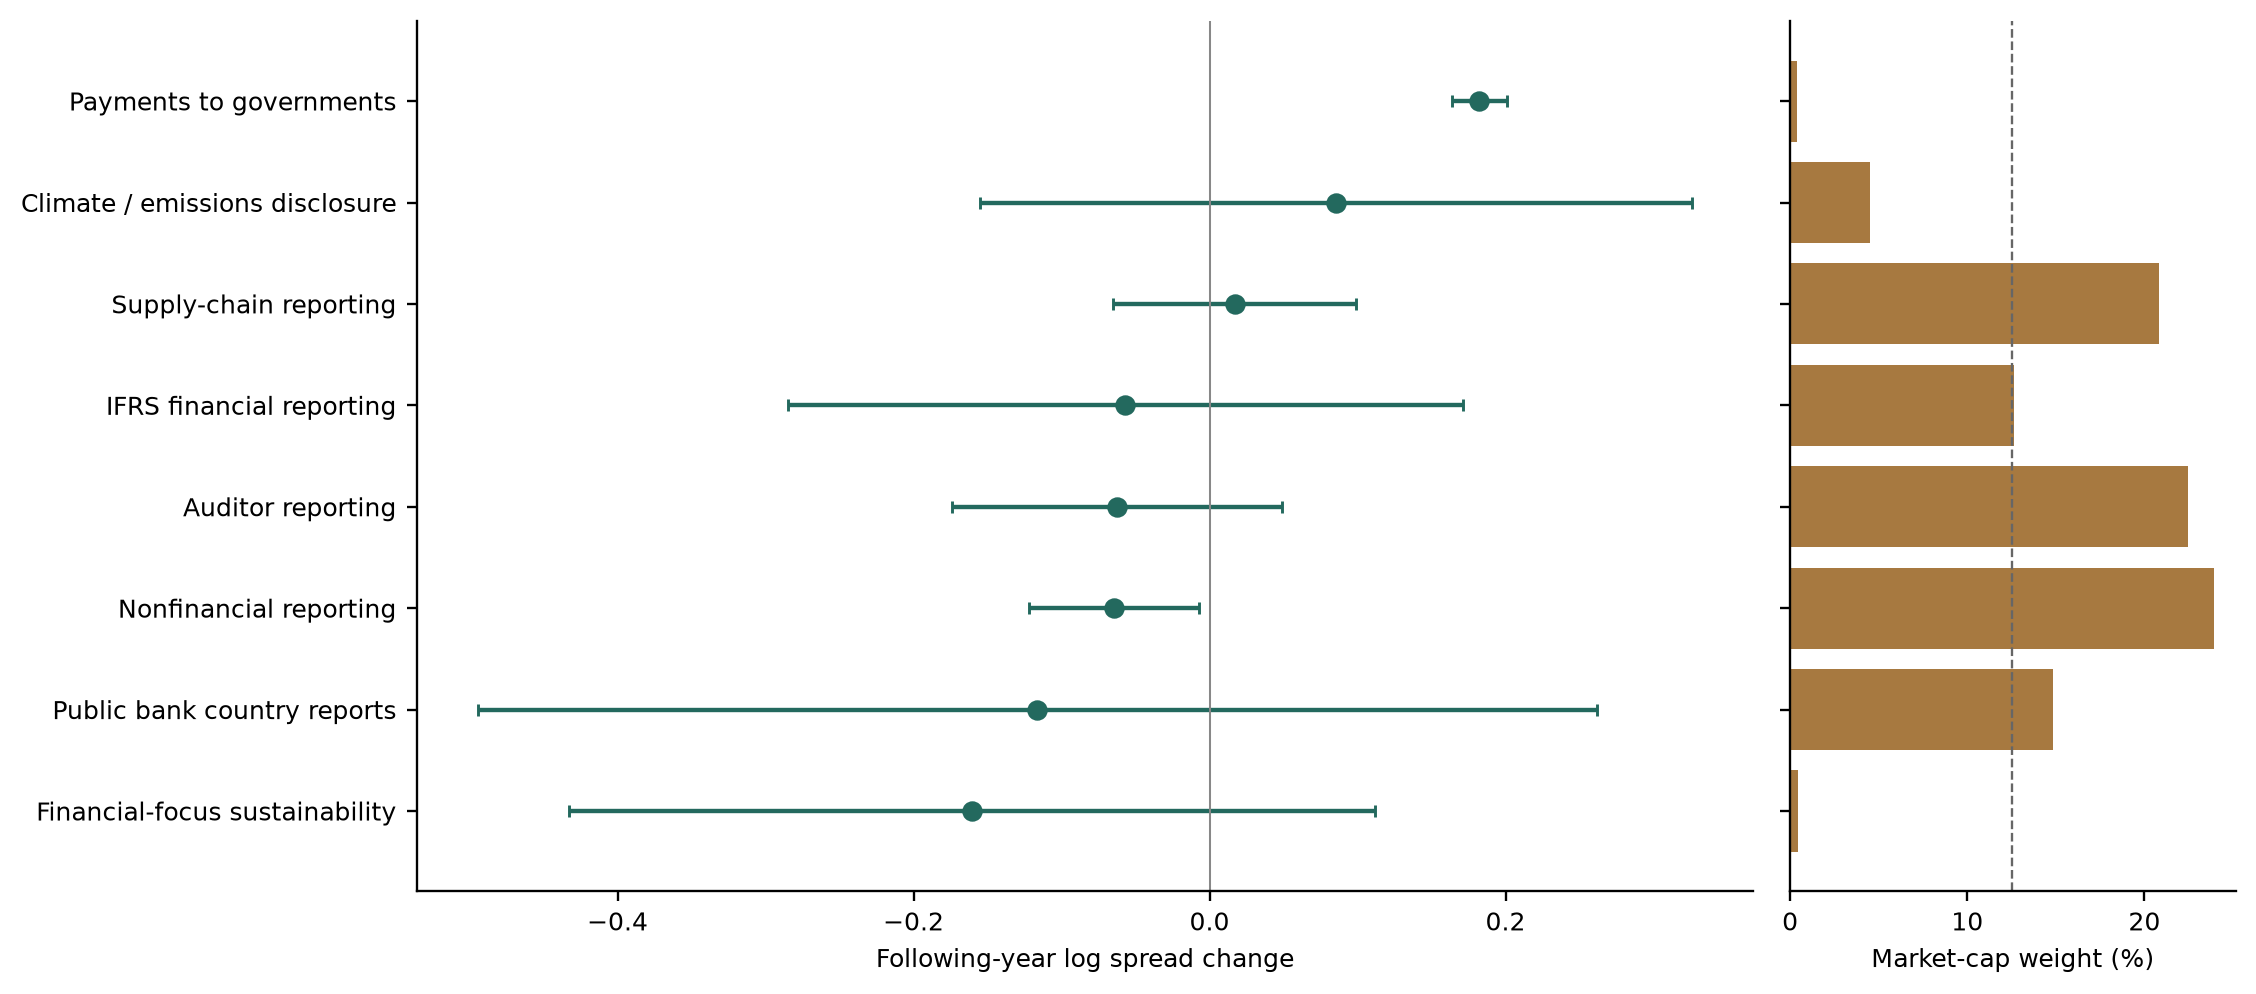
\includegraphics[width=\linewidth,height=0.72\textheight,keepaspectratio]{figure_tables/disclosure-family-effects.png}
\caption{Public-disclosure family estimates and weights}
{\footnotesize\raggedright Following-year GDP-weighted country comparisons. All eight supported families are shown. Bars are 95\% normal-reference conditional country intervals. Right panel: sampled pre-policy market-cap masses, normalised across these families; dashed line is equal family weight. Each family has its own supported countries and cohorts.\par}
\end{figure}

\clearpage\begin{figure}[p]\centering
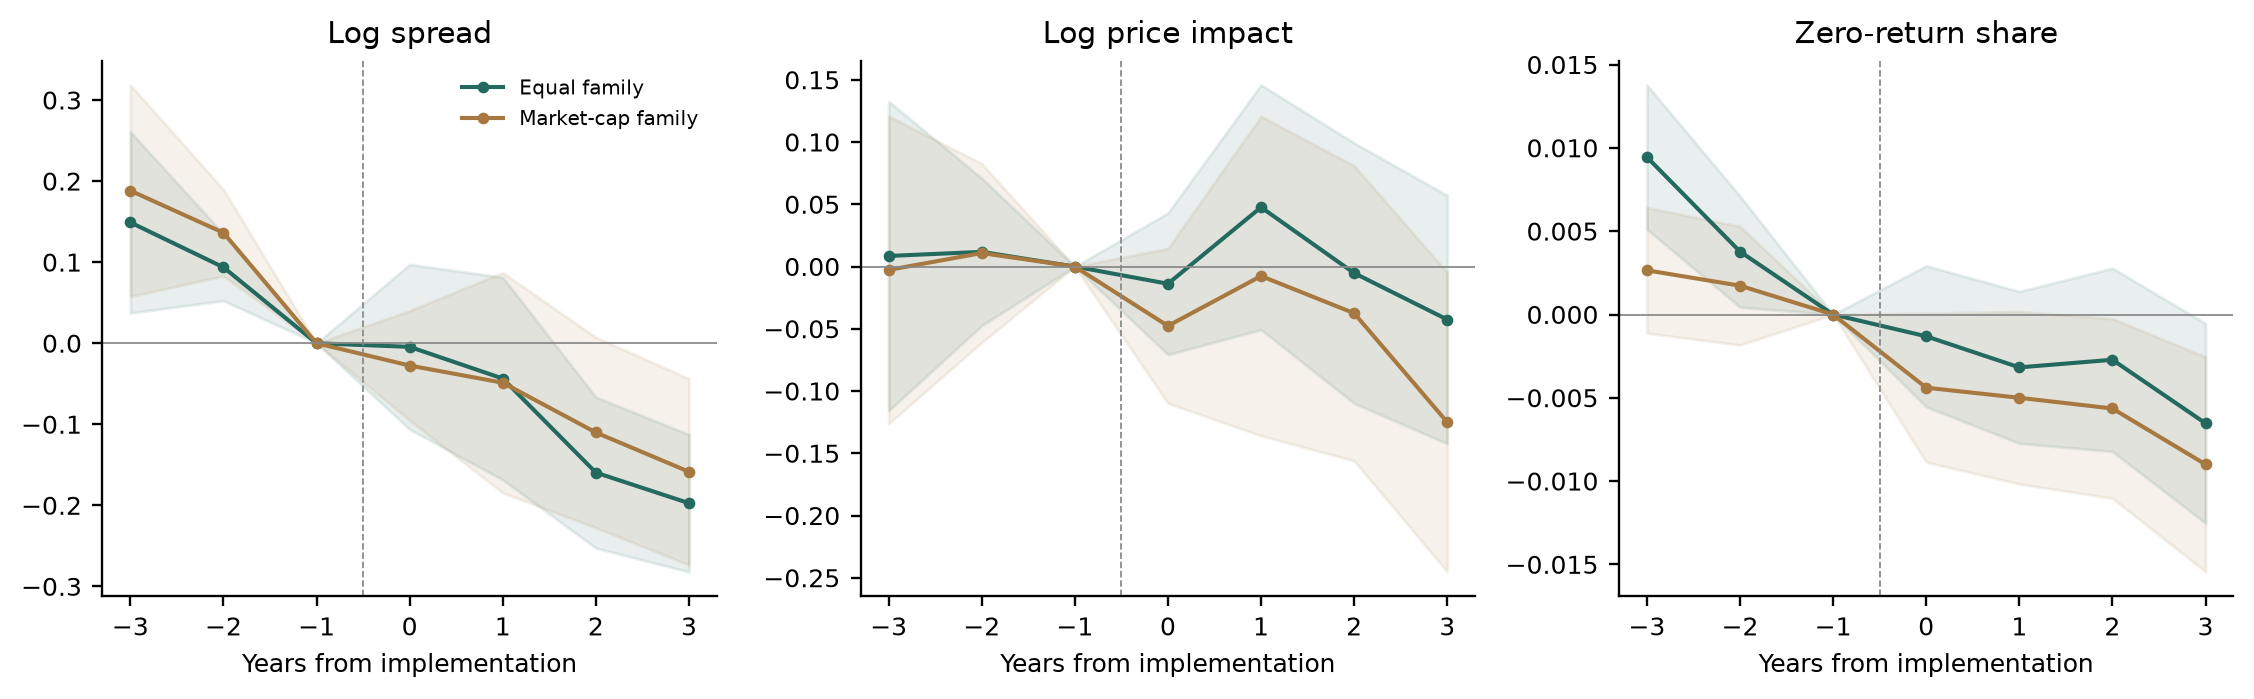
\includegraphics[width=\linewidth,height=0.72\textheight,keepaspectratio]{figure_tables/disclosure-event-profiles.png}
\caption{Public-disclosure liquidity before and after implementation}
{\footnotesize\raggedright Five public-disclosure families on fixed company support in years -3 through +3. Year -1 is the reference. Pointwise 95\% conditional country intervals are shaded. The sample differs from the eight-family short window and six-family longer-window main samples. Pre-policy differences and common legal waves limit a causal interpretation.\par}
\end{figure}

\clearpage\begin{figure}[p]\centering
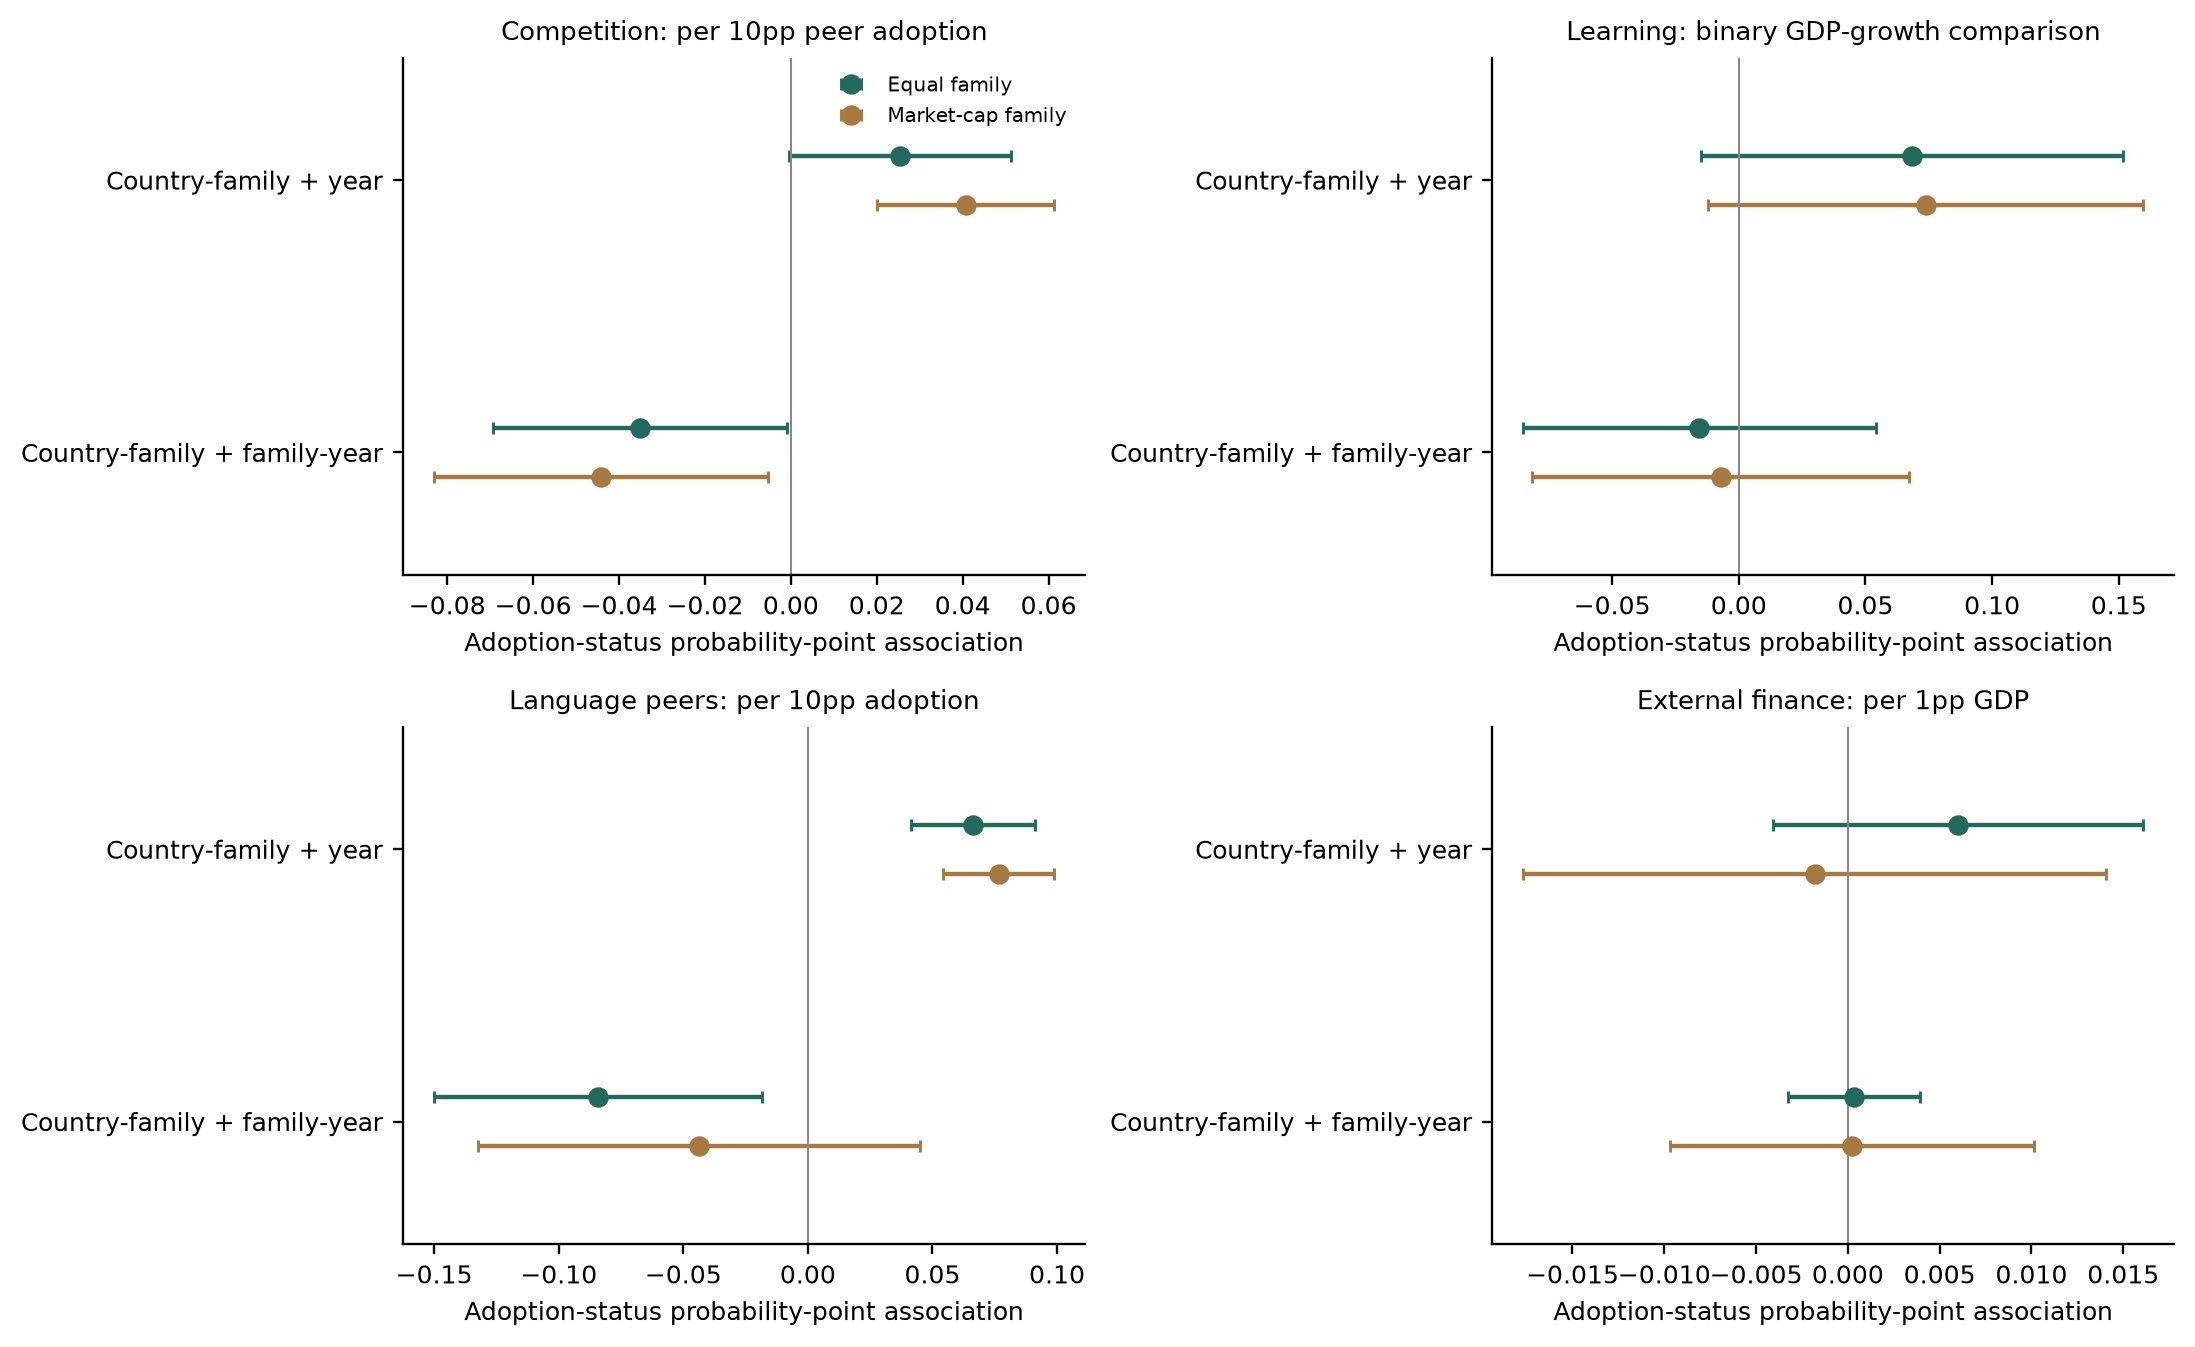
\includegraphics[width=\linewidth,height=0.72\textheight,keepaspectratio]{figure_tables/disclosure-diffusion-comparison.png}
\caption{Diffusion associations and common policy waves}
{\footnotesize\raggedright Separate adoption-status linear probability models under both family weights. Compare country-family plus common year effects with country-family plus family-year effects on identical rows. Horizontal intervals are 95\% country-clustered t intervals. Predictor units differ by panel and are stated in each heading. A change across fixed-effect structures is not evidence that either coefficient is causal.\par}
\end{figure}

\clearpage
\end{document}
